\ProvidesFile{ch-simulation.tex}[Light Curve Simulation]

\chapter{Light Curve Simulation}

Light curve simulation and inversion requires background knowledge in attitude kinematics, time and coordinate systems, computer graphics, and photometry. This section is broken into two major parts: simulating the object and its properties, and simulating the observations. The object simulation discussion proceeds with:

\begin{enumerate}
  \item Orbit and attitude propagation,
  \item Discrete mesh representations of shapes,
  \item Reflectance functions,
  \item Simulating light curves for convex objects,
  \item Simulating light curves for nonconvex objects.
\end{enumerate}

\noindent The discussion of the observation simulation proceeds with:

\begin{enumerate}
  \item Time and coordinate systems,
  \item Modeling the telescope sensor,
  \item Modeling the background,
  \item Observer constraints.
\end{enumerate}

This overall ordering for the simulation section of this work was chosen to promote an understanding of the object and its reflection properties in a simplified manner before expanding on the physics of the observer to introduce noise and accurate observation intervals to the light curve. To preface this section, the light curve and its common units must first be defined.

\subsection{The Light Curve}

The light curve expresses the observed brightness of an object over time. In literature, that brightness is commonly expressed in terms of irradiance, apparent magnitude, or photoelectron counts. These units are discussed in Section \ref{sec:brightness_units} This work also considers the normalized irradiance for some simulation and inversion tasks. Converting between these representations is accomplished with Eqs \ref{eq:count_to_irrad} and \ref{eq:irradiance_to_mag}.

\begin{figure}[!htb]
  \centering
  \includegraphics[width=\figbig]{sphx_glr_light_curve_units_001_2_00x.png}
  \caption{Synthetic light curves in counts, irradiance, normalized irradiance, and apparent magnitude}
  \label{fig:light_curve_units}
\end{figure}

Figure \ref{fig:light_curve_units} details this equivalence with the same light curve expressed in these four unit systems. This figure also displays an important characteristic of real measured light curves: they are always contaminated with noise. As a result, the "true mean" signal in Figure \ref{fig:light_curve_units} cannot be obtained through the raw measurements, and is merely computed here as a stepping stone to the measured digital signal in the CCD. The sources of this noise are described in detail in Section \ref{sec:ccd_performance}.

\section{Simulating Space Object Dynamics and Properties}

\subsection{Orbit Propagation}

There are many environmental perturbations that influence the natural motion of space objects in orbits around Earth. In LEO, drag and the $J_2$ term of Earth's gravity field due to equatorial oblateness are the dominant perturbations \cite{frueh2019notes}. In MEO and GEO, solar radiation pressure (SRP) and the third-body effects of the Sun and Moon become increasingly important while drag is negligible \cite{frueh2019notes}. For the purposes of accurate light curve simulation, the orbit propagation must be accurate enough for the hour to week-long scenarios, and it should also be easy to access real initial conditions for objects of interest near the propagation dates. To access historical and predicted trajectories of real space objects in the public catalog, Two-Line Element sets (TLEs) are used. TLEs are short, standardized collections of orbital elements and mission information, produced from observations of the object in question close to the publication date \cite{vallado4ed}. TLEs are available programmatically through Space-Track, a service provided by the US Space Force's 18th Space Defense Squadron \cite{spacetrack}. The Simplified General Perturbations 4 (SGP4) propagator is used to propagate near-Earth objects from TLEs. SGP4 models the secular effects of the first few zonal terms of Earth's gravity field, drag through an exponential density atmosphere, and some of the effects of third bodies like the Sun and Moon \cite{vallado4ed}. It should be noted that an improved propagator known as SGP4-XP has been developed to better model SRP, cislunar objects, gravitational harmonics, and atmospheric drag \cite{payne2022}. TLEs for SGP4-XP and SGP4 are not interchangeable \cite{payne2022}. The SGP4 propagator takes as input a Two-Line Element (TLE) set along with the Julian dates to propagate the object to and returns the position and velocity in the True Equator, Mean Equinox reference frame described in Section \ref{sec:teme} \cite{vallado4ed}. While SGP4 does not model some important perturbations like SRP, the availability of frequently updated TLEs for regularly tracked objects alleviates most concerns, although errors on the order of a few kilometers are still expected for LEO objects \cite{vallado4ed}. 

Orbital propagation for the simulations performed in this work was done using SGP4 with TLE interpolation. For a given set of Julian dates and the satellite name in question, Space-Track is queried to find all TLEs produced for that object in the interval of interest. SGP4 is run for all Julian dates and all TLEs, and the final position at each Julian date is linearly interpolated between the most recent past TLE and the next future TLE. If there is only one neighboring TLE, its position is used without interpolation.

\subsection{Attitude Propagation}

In order to effectively compute reflections and shadows on the surfaces of space objects, that object must have an assigned orientation in inertial space. While defunct satellites and space debris are slowly spun up by the Yarkovsky-O'Keefe-Radzievskii-Paddack (YORP) effect, the short-term motion of non-operational space objects is well-approximated by torque-free motion \cite{benson2018cyclic}. Developing the kinematics of torque-free motion first requires an understanding of common kinematic representations of orientation.

The orientation --- or attitude --- of a rigid body in three dimensions is implicitly understood to be relative to some other reference frame. The direction of a unit vector can be expressed with two numbers ---  the azimuth and elevation of that vector. Naively, this could be extrapolated to conclude that six numbers are needed to express an orientation. Because the basis vectors form an orthonormal set $\left\{ \hat{b}_1, \hat{b}_2, \hat{b}_3\right\}$, it follows for a right-handed system that $\hat{b}_3 = \hat{b}_1 \times \hat{b}_2$, $\hat{b}_2 = \hat{b}_3 \times \hat{b}_1$, and $\hat{b}_1 = \hat{b}_2 \times \hat{b}_3$. Each of these equations constrains one further degree of freedom, revealing that a minimum of three quantities are necessary to express the relative orientation of two reference frames. This minimum bound does not make any statements about the usefulness of three element sets; at least four dimensions are needed to remove singularities \cite{crassidis1ed}.

\subsubsection{The Direction Cosine Matrix}

The direction cosine matrix (DCM) is a $3\times3$ symmetric, orthogonal matrix, expressing the three basis vectors of one frame in another. This amounts to projecting each basis vector in the first frame onto each basis vector of the second frame --- the cosine of the angle between the compared vectors. It is notated with two capital letters, the rightmost indicating the reference frame of the input vectors and the leftmost indicating the transformed frame. Alternatively, the DCM is sometimes expressed as $C$ when the frames involved are arbitrary or do not need to be denoted. For example, the DCM $\dcm{bn}$ takes a vector $\vrf{n}{r}$ in the $\rf{n}$ frame to the $\rf{b}$ frame as $\vrf{b}{r}$ \cite{shuster1993}:

\begin{equation}
    \vrf{b}{r} = \dcm{bn} \vrf{n}{r}.
\end{equation}

The orthogonal property of the DCM implies $\dcm{bn}^{-1} = \dcm{bn}^T$ such that $\dcm{bn}^T = \dcm{nb}$ \cite{shuster1993}. 

\subsubsection{Principal Rotation Parameters}

Another common attitude representation is the Euler angle-axis set, otherwise known as principal rotation parameters \cite{crassidis1ed}. Euler's rotation theorem guarantees that any relative orientation can be expressed as a single rotation about an axis $\hat{\lambda} \in \mathbb{S}^2$ by an angle $\theta \in [0, 2\pi]$ \cite{crassidis1ed}. The set $\left\{\hat{\lambda},\theta\right\}$ is known as a principal rotation parameter, abbreviated PRP hereafter. The DCM is mapped to the PRP representation with \cite{shuster1993}:

\begin{align*} \numberthis \label{eq:dcm_to_prp}
    \theta &= \cos^{-1}\left(\frac{1}{2} \left[C_{11} + C_{22} + C_{33} - 1 \right] \right), \\
    \hat{\lambda} &= \frac{1}{2\sin{\theta}} 
    \begin{bmatrix} C_{23} - C_{32} \\ C_{31}-C_{13} \\ C_{12} - C_{21}\end{bmatrix},
\end{align*}

where $C_{i,j}$ refers to the $i$th row and $j$th column of $C$ \cite{shuster1993}. The mapping from PRP to DCM is also relatively straightforward \cite{shuster1993}:

\begin{equation} \label{eq:prp2dcm}
    C = I_3 + \sin\theta\matcp{\hat{\lambda}} + (1-\cos\theta)\matcp{\hat{\lambda}}^2,
\end{equation}

were $I_3$ is the $\left[ 3 \times 3 \right]$ identity matrix and $\matcp{v}$ is the matrix cross product operator, defined on $\vctr{v} \in \mathbb{R}^3$ as \cite{shuster1993}:

\begin{equation}
    \matcp{\vctr{v}} = \begin{bmatrix}
        0 & -v_3 & v_2 \\
        v_3 & 0 & -v_1 \\
        -v_2 & v_1 & 0
    \end{bmatrix}.
\end{equation}

This operator is useful as it rephrases the cross product as matrix multiplication, i.\,e.\ $\vctr{v} \times \vctr{u} = \matcp{\vctr{v}}\vctr{u}$. While the PRP $\{\theta, \hat{\lambda}\}$ is a four element set, there are only three degrees of freedom due to the unit norm constraint on $\hat{\lambda}$. 

\subsubsection{Quaternions}

The quaternion represents attitude with a point on the surface of the hypersphere \sthree. In terms of the PRP, the quaternion is given by \cite{crassidis1ed}:

\begin{equation} \label{eq:prp2quat}
    \vctr{q} = \begin{bmatrix} \hat{\lambda} \sin\left( \frac{\theta}{2} \right) \\ \cos\left(\frac{\theta}{2}\right) \end{bmatrix}.
\end{equation}

The first three entries of the quaternion are often called the vector component, with the final entry being the scalar component. Some authors reorder the quaternion, placing the scalar term first. Often the entries of a single quaternion are referenced by index such that $\vctr{q} = \left[ q_1, q_2, q_3, q_4 \right]$. Similarly, the vector portion of the quaternion is referenced with $\vctr{q}_{1:3}$. The quaternion can be mapped back to the PRP \cite{crassidis1ed} via:

\begin{align*} \numberthis \label{eq:quat2prp_theta} 
    \theta &= 2 \cos^{-1}\left( q_4 \right) \\
    \hat{\lambda} &= \frac{\vctr{q}_{1:3}}{\sin{\frac{\theta}{2}}}.
\end{align*}

The quaternion maps to the DCM \cite{crassidis1ed} via:

\begin{equation} \label{eq:quat2dcm}
        C = \left[\begin{matrix}\ -\ q_2^2-\ q_3^2+q_1^2+q_4^2\ &\ 2\ q_1q_2+2\ q_3q_4&\ 2\ q_1q_3-2\ q_2q_4\\\ 2\ q_1q_2-2\ q_3q_4&\ -\ q_1^2-\ q_3^2+q_2^2+q_4^2\ &\ 2\ q_1q_4+2\ q_2q_3\\\ 2\ q_1q_3+2\ q_2q_4&\ 2\ q_2q_3-2\ q_1q_4&\ -q_1^2-\ q_2^2+q_3^2+q_4^2\\\end{matrix}\right]
\end{equation}

\subsection{Attitude Kinematics}

Quaternion kinematic differential equations are chosen for simulating object attitude profiles as they have no singularity and produce very smooth dynamics that are easy to integrate when compared to three-variable representations that possess singularities. Given the current orientation quaternion $\vctr{q} = [q_1, q_2, q_3, q_4]^T$ and angular velocity $\vctr{\omega} = [\omega_1, \omega_2, \omega_3]^T$ the quaternion derivative is computed via \cite{crassidis1ed}:

\begin{equation} \label{eq:quat_kde}
    \left[\begin{matrix}\dot{q}_1\\\dot{q}_2\\\dot{q}_3\\\dot{q}_4\\\end{matrix}\right]
    =
    \frac{1}{2}\left[\begin{matrix}q_4&-q_3&q_2&q_1\\q_3&q_4&-q_1&q_2\\-q_2&q_1&q_4&q_3\\-q_1&-q_2&-q_3&q_4\\\end{matrix}\right]
    \left[\begin{matrix}\omega_1\\\omega_2\\\omega_3\\0\\\end{matrix}\right].
\end{equation} 

\subsection{Attitude Dynamics}

Rigid body dynamics can be easily expressed in the body principal axes for an object with the diagonal inertia tensor $J = \mathrm{diag}\left( J_1, J_2, J_3 \right)$ with an arbitrary torque $\vctr{M} = \left[M_1, M_2, M_3\right]^T$ in the same frame via \cite{crassidis1ed}:

\begin{equation} \label{eq:rbtf_dynamics}
    \left[\begin{matrix}\dot{\omega_1}\\\dot{\omega_2}\\\dot{\omega_3}\\\end{matrix}\right]
    =
    \left[\begin{matrix}
        \left(M_1+J_2\omega_2\omega_3-J_3\omega_2\omega_3\right) / J_1 \\
        \left(M_2-J_1\omega_1\omega_3+J_3\omega_1\omega_3\right) / J_2 \\
        \left(M_3+J_1\omega_1\omega_2-J_2\omega_1\omega_2\right) / J_3 \\
    \end{matrix}\right].
\end{equation}

Equations \ref{eq:rbtf_dynamics} and \ref{eq:quat_kde} are numerically integrated to yield the orientation time history which is necessary for later light curve simulations. Often, $\vctr{M} = \mathbf{0}$ is chosen to simulate the torque-free evolution of an initial orientation and spin state, neglecting small attitude perturbations over the simulation interval.

\subsection{Discrete Shape Representations}

A computer can represent 3D objects implicitly or explicitly. An implicit representation might be the solution to an algebraic equation, i.\,e.\, $x^2 + y^2 + z^2 = 1$ defines a sphere of radius $1$ centered at the origin. Often, a shape may be defined by a set of signed distance functions (SDFs). An SDF takes in a point in \rthree and outputs the distance from the object, returning negative distance if the queried point is inside the shape. The object can then be rendered via ray marching. A ray is cast from the camera out into the scene for each pixel of the screen, each performing distance queries along its length until it intersects the object or diverges. 

By contrast, an explicit shape representation creates complex 3D geometry from simple 2D building blocks. In the most common case, object faces are defined by triangles. This means that at the scale of the individual faces, the shape is always composed of flat surfaces that meet at sharp angles. While this can add complexity to many fields of shape analysis and geometry processing, triangulated surfaces are perfect for light curve shape inversion. Human-made space objects like most satellites are composed of flat faces, with the exception of parabolic antennas and cylindrical rocket bodies.

\subsubsection{The Object File Format}

One common text file format for 3D model files is \texttt{.obj}, developed by Wavefront Technologies in the early 1990s \cite{obj_format}. Each OBJ file consists of a list of vertex positions and face definitions, with optional vertex normals and tangents. An \texttt{.obj} listing for a cube is included for reference in Appendix \ref{sec:obj_listing}. Given the vertex positions and adjacency information stored in the model file, useful properties of the object can be computed for use later in both light curve simulation and shape inversion. 

\subsubsection{Properties of Triangulated Meshes}

For each triangular face $F_i$ of the model defined by vertices $F_i = \left\{v_1, v_2, v_3\right\}$, the outward-pointing face normal is computed with:

\begin{equation} \label{eq:face_normal}
    \vctr{n} = \frac{\left( v_2 - v_1 \right) \times \left( v_3 - v_1 \right)}{\| \left( v_2 - v_1 \right) \times \left( v_3 - v_1 \right) \|_2}.
\end{equation}

The face area is computed with:

\begin{equation} \label{eq:face_areas}
    a = \frac{\| \left( v_2 - v_1 \right) \times \left( v_3 - v_1 \right)\|_2}{2}.
\end{equation}

The support of the $i$th face --- the perpendicular distance from the origin to the plane defining the face --- is computed with the position of any vertex on that face, i.\,e.\, the first vertex $v_{i,1}$, and the face normal vector $\vctr{n}_i$:

\begin{equation} \label{eq:face_support}
    h_i = v_{i,1} \cdot \vctr{n}_i.
\end{equation}

The volume of the object is computed:

\begin{equation} \label{eq:object_volume}
    V = \frac{1}{3} \sum_{i=0}^{ \lvert F \rvert}\vctr{h}_i \cdot \vctr{a}_i.
\end{equation}

In Eq \ref{eq:object_volume}, $\lvert F \rvert$ is the number of faces defining the object. $\vctr{h}$ and $\vctr{a}$ are column vectors collecting all face supports and areas. The Extended Gaussian Image, a quantity defined in \ref{sec:egi_definition}, is computed row-wise for the $i$th face with:

\begin{equation} \label{eq:egi_definition}
    \vctr{E}_i = \vctr{a}_i \vctr{n}_i.
\end{equation}

\subsection{The Bidirectional Reflectance Distribution Function}

Although light curves come from unresolved measurements, the interactions that produce them are directly driven by the shape and material properties of the object being observed. In order to simulate accurate light curves, all relevant optical interactions must be modeled. In broad terms, this boils down to determining how the object is illuminated, how it casts shadows on itself, and how it is observed. 

At the microscopic scale, the surface of an object is composed of facets ---  small areas sharing a normal vector. The macroscopic optical properties of the material is driven by the distribution of sizes and normal directions of these microfacets. If the facet normals are distributed in biased orientations, the macroscopic surface may show anisotropy, leading to the appearance of brushed metal. If the microfacet normals are at large angles to each other, the surface may appear dull as the direction of the outgoing light may be largely independent from the incoming direction. Subsurface effects ---  where incoming light rays scatter \textit{inside} the surface --- can also change the macroscopic properties of the material. 

This discussion raises an important question; how should the macroscopic outcomes of the microscopic interactions of incident light on a surface be modeled? The bidirectional reflectance distribution function (BRDF) is a tool from computer graphics that addresses this problem. The BRDF is a function on the hemisphere which expresses the fraction of light per solid angle (radiance $\mathcal{R}$) leaving the surface in a given direction, divided by the incident power per unit area (irradiance $\mathcal{I}$). The general formulation for a BRDF $f_r$ is given by \cite{duvenhage2013}:

\begin{equation} \label{eq:brdf_def}
    f_r(\vctr{x}, L, O) = \frac{d\mathcal{R}\left(\vctr{x}, O\right)}{d\mathcal{I}\left(L, \vctr{x}\right)}.
\end{equation}

In Eq \ref{eq:brdf_def}, $\vctr{x} \in \mathbb{R}^3$ is the point on the object's surface where the BRDF is evaluated. $\vctr{\ell} \in \mathbb{S}^2$ is the incoming illumination unit vector and $\vctr{o} \in \mathbb{S}^2$ is the outgoing unit vector. Note that this work treats $f_r(\vctr{x}, \vctr{\ell}, \vctr{o})$ and $f_r(\vctr{\ell}, \vctr{o})$ as equivalent in later descriptions, leaving the evaluation point $\vctr{x}$ implied. This definition is useful for building intuition about the form of the BRDF, but to represent a physically plausible reflection process, a candidate function must satisfy three additional constraints. A physically plausible BRDF must conserve energy --- more energy cannot be reflected from the surface than was incident on it. It must also be reciprocal --- switching the observer and illumination directions should not change the BRDF value as the surface interaction. This reciprocity is sometimes known as the \textit{Helmholtz Reciprocity Rule} in literature \cite{montes2012}. Finally, plausible BRDFs are positive --- they take on nonnegative values for all valid inputs \cite{montes2012}. A surface cannot reflect negative light, so this is expected. Explicitly, energy conservation is expressed with \cite{montes2012}:

\begin{equation} \label{eq:brdf_energy_cons}
  \forall \vctr{\ell} \in \mathbb{S}^2 : \:\: \int_{\vctr{o} \in \mathbb{S}^2} f_r(\vctr{\ell}, \vctr{o}) \: d\mathbb{S}^2 \leq 1.
\end{equation}

Eq \ref{eq:brdf_energy_cons} states that for all possible illumination directions $L$, integrating all possible outgoing observer directions $O$ on the unit sphere cannot return greater than one from the energy conservation integral. Reciprocity can be formalized as:

\begin{equation} \label{eq:brdf_reciprocity}
  \forall \vctr{\ell}, \vctr{o} \in \mathbb{S}^2 : \:\: f_r(\vctr{\ell}, \vctr{o}) = f_r(\vctr{o}, \vctr{\ell}).
\end{equation}

Now that the requirements for a plausible physical BRDF have been established, a collection of commonly-used BRDFs can be presented. The following BRDFs are all energy conserving, reciprocal, and nonnegative. Real-world materials are modeled with these BRDFs by fitting the free parameters of a given BRDF to measured reflectance data \cite{matusik2003}. If a BRDF can be fit to the data with low error, that reflection function can be considered to be a faithful model for the true physics. 

\subsubsection{Lambertian}

The simplest BRDF is one that reflects equally in all directions. This BRDF is termed Lambertian or diffuse.

\begin{equation} \label{eq:brdf_lambertian}
  f_r(\vctr{\ell}, \vctr{o}) = \frac{C_d}{\pi}
\end{equation}

In Eq \ref{eq:brdf_lambertian}, $0 \leq C_d \leq 1$ is the surface's coefficient of diffuse reflection. For example, $C_d = 0.4$ means that the surface reflects $40\%$ of incident radiation and absorbs the other $60\%$. 

While the diffuse BRDF reflects energy isotropically, many real-world reflections are highly biased. At the extreme end, a perfect mirror reflection is effectively a Dirac delta function in the reflected illumination direction. Many real-world materials are well modeled as a linear combination of diffuse and specular effects. 

\subsubsection{Phong}

A simple specular BRDF model is that developed by Phong in 1975 \cite{phong1975}. The Phong model splits the BRDF into a Lambertian term governed by $C_d$ and a specular term governed the coefficient of specular reflection $ 0 \leq C_s \leq 1$ and the specular exponent $n \geq 0$ \cite{duvenhage2013}. 

\begin{equation} \label{eq:brdf_phong}
  f_r(\vctr{\ell}, \vctr{o}) = \frac{C_d}{\pi} + \frac{C_s \frac{n+2}{2\pi} (\vctr{o} \cdot \vctr{R})^n}{\vctr{n} \cdot \vctr{\ell}}
\end{equation}

In Eq \ref{eq:brdf_phong}, $\vctr{R}$ is the reflected illumination vector, computed via $\vctr{R} = 2 (\vctr{n} \cdot \vctr{\ell}) \vctr{n} - \vctr{\ell}$. As $n$ increases, the specular glint becomes sharper and more intense, eventually approaching a perfect mirror reflection. Because of the introduction of a new coefficient of reflection, a new constraint is needed to maintain energy conservation. Because $C_d$ and $C_s$ each represent the \textit{fraction} of light reflected in each mode, it should be clear that $C_d + C_s \leq 1$. This can also be reformulated with an explicit coefficient of absorption $C_a$ which captures the fraction of incident radiation absorbed by the surface, yielding $C_d + C_s + C_a = 1$. It must be noted that the Phong model is only approximately reciprocal as it is based on the reflected incident vector $\vctr{R}$ instead of the halfway vector $\vctr{H}$ used by other models \cite{duvenhage2013}.

\subsubsection{Blinn-Phong}

The Blinn-Phong BRDF is similar to the Phong BRDF, but it parameterizes the specular lobe in terms of the halfway vector $\vctr{H}$ \cite{duvenhage2013}. This vector is halfway between the illumination and observer directions such that $\vctr{H} = \vctr{\ell} + \vctr{o}$ which needs to be normalized before use. As the halfway vector approaches the surface normal vector, the observer must be approaching the reflected illumination vector, leading to a more intense specular highlight. 

\begin{equation} \label{eq:brdf_blinn_phong}
  f_r(\vctr{\ell}, \vctr{o}) = \frac{C_d}{\pi} + \frac{C_s \frac{n+2}{2\pi} (\vctr{n} \cdot \vctr{H})^n}{4 (\vctr{n} \cdot \vctr{\ell})(\vctr{n} \cdot \vctr{o})}
\end{equation}

\subsubsection{Glossy}

The so-called glossy BRDF simulates reflections from plastic materials using an Gaussian distribution around the specular scattering lobe \cite{duvenhage2013}:

\begin{equation} \label{eq:brdf_glossy}
  f_r(\vctr{\ell}, \vctr{o}) = \frac{C_d}{\pi} + \frac{C_s}{2\pi \sigma^2 \left(N \cdot L\right)}  e^{\frac{-\left( R \cdot O \right)^2}{2\sigma^2}},
\end{equation}

where the parameter $\sigma$ controls the width of the specular Gaussian. It must be noted that the Glossy model is only approximately reciprocal as it is based on the reflected incident vector $\vctr{R}$ instead of the halfway vector $\vctr{H}$ used by other models \cite{duvenhage2013}.

\subsubsection{Cook-Torrance}

The Cook-Torrance explicitly accounts for the orientation of the microfacets making up the surface \cite{cook1982}. This model is built from a facet slope distribution term $D_{ct}$, a Fresnel term $F$, and a geometric attenuation factor $G_{ct}$. The slope distribution term describes the probability density of a given facet being oriented with a normal vector aligned with the halfway vector $\vctr{H}$ \cite{cook1982}. A common formulation of this term is due to Beckmann:

\begin{equation} \label{eq:d_beckmann}
  D_{ct} = \frac{1}{\pi \alpha^2 \left( \vctr{n} \cdot \vctr{H} \right)^4} \exp\left( \frac{1 - \left(\vctr{n} \cdot \vctr{H}\right)^2}{\alpha^2 \left( \vctr{n} \cdot \vctr{H} \right)^2} \right).
\end{equation}

In Eq \ref{eq:d_beckmann}, $\alpha \in [0, 1]$ is the roughness of the surface \cite{cook1982}. The Fresnel term accounts for the variation in specular reflection due to the angle of incidence. In reality, this term is a function of wavelength, but it is often approximated as \cite{cook1982}:

\begin{equation} \label{eq:fresnel_approx}
  F = C_s + \left( 1 - C_s \right) \left( 1 - \left( \vctr{H} \cdot \vctr{\ell} \right) \right) ^ 5.
\end{equation}

The geometric attenuation term expresses how microfacets shadow each other, and can be approximated with \cite{cook1982}:

\begin{equation} \label{eq:cook_torrance_g}
  G_{ct} = \min \left\{ 1, \frac{2\left(\vctr{n} \cdot \vctr{H}\right) \left(\vctr{n} \cdot \vctr{o} \right)}{\vctr{o} \cdot \vctr{H}}, \frac{2\left(\vctr{n} \cdot \vctr{H}\right) \left(\vctr{n} \cdot \vctr{\ell}\right)}{\vctr{o} \cdot \vctr{H}} \right\}.
\end{equation}

The overall reflectance for the Cook-Torrance BRDF is given by:

\begin{equation} \label{eq:brdf_cook_torrance}
  f_r(\vctr{\ell}, \vctr{o}) = \frac{C_d}{\pi} + \frac{D_{ct} \cdot G_{ct} \cdot F}{4 \left(\vctr{n} \cdot \vctr{\ell}\right) \left( \vctr{n} \cdot \vctr{o} \right)}
\end{equation}

\subsubsection{Oren-Nayar}

The Oren-Nayar BRDF is an improved model of diffuse reflectance for many real-world materials like ceramics and the surface of the Moon. These materials diverge from the Lambertian model near the horizon, reflecting much more light than would be predicted by simple cosine loss \cite{oren1994}. This BRDF relies on the surface roughness $\alpha$ to compute a set of constants \cite{oren1994}:

\begin{align*} \numberthis
  A &= 1 - 0.5 \frac{\alpha^2}{\alpha^2 + 0.33} \\
  B &= 0.45 \frac{\alpha^2}{\alpha^2 + 0.09} \\
  C &= \frac{\mathrm{proj}_{\vctr{n}}\left(\vctr{\ell}\right)}{\|\mathrm{proj}_{\vctr{n}}\left(\vctr{\ell}\right)\|} \cdot  \frac{\mathrm{proj}_{\vctr{n}}\left(\vctr{o}\right)}{\|\mathrm{proj}_{\vctr{n}}\left(\vctr{o}\right)\|} \\
  \beta &= \max \left\{ \cos^{-1}\left( \vctr{\ell} \cdot \vctr{n} \right), \: \cos^{-1}\left( \vctr{o} \cdot \vctr{n} \right) \right\} \\
  \gamma &= \min \left\{ \cos^{-1}\left( \vctr{\ell} \cdot \vctr{n} \right), \: \cos^{-1}\left( \vctr{o} \cdot \vctr{n} \right) \right\}. \\
\end{align*}

With these values computed, the reflectance of the Oren-Nayar BRDF is given by \cite{oren1994}:

\begin{equation}
  f_r(\vctr{\ell}, \vctr{o}) = \frac{C_d}{\pi} \left(A + (B \max\left\{C, 0\right\} \sin\beta \tan\gamma) \right).
\end{equation}

\subsubsection{Ashikhmin-Shirley}

The Ashikhmin-Shirley BRDF is unique among those presented in this section as it allows for anisotropic reflection which can be non-negligible for metals \cite{ashikhmin2000}. This model is parameterized by the diffuse reflection coefficient, as well as two specular exponents $n_u$ and $n_v$. When $n_u = n_v$, the model behaves much like the Phong BRDF. The full BRDF is expressed \cite{ashikhmin2000}:

\begin{align*} \numberthis \label{eq:brdf_ashikhmin_shirley}
  \rho_d &= \frac{28 C_d}{23 \pi} (1 - C_s) \left(1 - \left(1 - \frac{\vctr{n} \cdot \vctr{\ell}}{2}\right)^5\right) \left(1 - \left(1 - \frac{\vctr{n} \cdot \vctr{o}}{2}\right)^5\right) \\
  \rho_s &= \frac{\sqrt{(n_u+1)(n_v+1)}}{8 \pi} \frac{\left( \vctr{n} \cdot \vctr{H} \right)
  ^\frac{n_u \left(\vctr{H} \cdot \vctr{U} \right)^2 + n_v \left( \vctr{H} \cdot \vctr{V} \right)^2}{1 - \left(\vctr{H} \cdot \vctr{n}\right)^2}}
  {\left(\vctr{H} \cdot \vctr{\ell}\right) \max\left\{ \vctr{n} \cdot \vctr{o}, \vctr{n} \cdot \vctr{\ell} \right\}} F \\
  f_r(\vctr{\ell}, \vctr{o}) &= \rho_d + \rho_s. \\
\end{align*}

In Eq \ref{eq:brdf_ashikhmin_shirley}, $F$ is the same Fresnel factor in Eq \ref{eq:fresnel_approx} while $U$ and $V$ are predefined surface basis vectors perpendicular to the surface normal.

\subsection{BRDF Summary}

\begin{figure}[ht]
  \centering
  \includegraphics[width=\figbig]{sphx_glr_brdf_renders_002_2_00x.png}
  \caption{Implemented BRDFs rendered with arbitrary parameters, demonstrating the qualitative differences between lighting models}
  \label{fig:brdf_renders}
\end{figure} 

\subsection{Real Material Properties}

Producing accurate light curves requires accurate optical properties for the simulated materials. Matusik et al.\ compiled measured bidirectional reflectance data from over 100 real materials including various metals and paints that might be found on human-made space objects \cite{matusik2003}. Optimally, such a dataset would be used to model the structure, solar panels, and antenna surfaces of the simulated objects. However, it is far more computationally efficient to fit one of the presented three parameter BRDFs to observed data. The Phong model parameters used for simulations in this work are listed in Table \ref{tb:real_matprops}.

\begin{table}[]
  \centering
  \begin{tabular}{|l|l|l|l|}
  \hline
  \textbf{Material} & $C_d$ & $C_s$ & $n$ \\ \hline
  Solar panel (Phong) \cite{fankhauser2023}              & $0.15$ & $0.25$ & $0.26$  \\ \hline
  Bus structure (Phong) \cite{fankhauser2023}               & $0.34$ & $0.40$ & $8.9$  \\ \hline
  Multilayer insulation (MLI) (Phong) & $0.1$ & $0.9$ & $20$ \\ \hline
  White paint (Phong) & $0.9$ & $0.1$ & $1$ \\ \hline
  \end{tabular}
  \caption{Reflection properties of real materials. MLI and white paint parameters are estimated qualitatively by the author. Significant variance may exist between objects depending on surface finishes \cite{matusik2003}.}
  \label{tb:real_matprops}
\end{table}

\subsection{Brightness Units} \label{sec:brightness_units}

\subsubsection{Irradiance}

Irradiance is the standard SI linear unit used to describe the total amount of energy incident on a
surface from a given source. An irradiance of $1 \: \left[ \frac{W}{m^2} \right]$ implies that a $10
\: [m^2]$ area would experience $10 \: [W]$ of incident power. The mean irradiance of the Sun --- termed the solar constant --- is derived from the mean luminosity of the Sun $L_s = 3.828\cdot10^{26} \: [W]$ and a distance of $1$ Astronomical Unit $1 \: [AU] = 149597870.7 \: [km]$ \cite{frueh2019notes}. The mean solar constant is then computed via

\begin{equation} \label{eq:solar_constant_mean}
  I_s = \frac{L_s}{4\pi \left(AU\right)^2} \approx 1361.0 \: \left[ \frac{W}{m^2} \right].
\end{equation}

In reality, the exoatmospheric irradiance at Earth varies \cite{frueh2019notes}. Figure \ref{fig:tsi} displays the small variations in the solar irradiance due to the solar cycle and the much larger variations due to Earth's eccentric orbit.

\begin{figure}[ht]
  \centering
  \includegraphics[width=\figmed]{sphx_glr_total_solar_irradiance_003_2_00x.png}
  \caption{Total solar irradiance variations at Earth and 1 AU. The solar cycle is apparent when distance is held constant at 1 AU, yielding small variations in the peak intensity at Earth.}
  \label{fig:tsi}
\end{figure}

\subsubsection{Apparent Magnitude}

Apparent magnitude ---  also known as visual or relative magnitude --- is a reverse logarithmic scale
that originates in astronomy \cite{frueh2019notes}. Stellar sources span many orders of magnitude of brightness, making a
logarithmic scale a helpful middle ground for comparison. Note that apparent magnitude always
expresses brightness at the observer's location; absolute magnitude is a different quantity that
normalizes brightness from a distance of $10$ parsecs \cite{frueh2019notes}. Apparent magnitude $m$
is computed from irradiance via \cite{frueh2019notes}:

\begin{equation} \label{eq:irradiance_to_mag}
  m = -2.5 \log_{10}\left( \frac{I}{I_0} \right).
\end{equation}

In Eq \ref{eq:irradiance_to_mag}, $I$ is the irradiance of the source of interest and $I_0$ is
irradiance of the zero-point source. This makes sense; substituting $I = I_0$ returns
$m=0$. The star Vega is usually taken to be the zero-point with irradiance $I_0 = 2.518021002\cdot
10^{-8} \: \left[ \frac{W}{m^2} \right]$ \cite{frueh2019notes}.

Eq \ref{eq:irradiance_to_mag} is rearranged to compute irradiance from a given apparent magnitude,
yielding:

\begin{equation} \label{eq:mag_to_irradiance}
  I = I_0 \cdot 10^{-\frac{m}{2.5}}.
\end{equation}

\subsubsection{Normalized Irradiance}

The light curve simulation methods presented in this work use normalized irradiance, the received irradiance of an object at a distance of $1$ meter per $\left[ W/m^2 \right]$ of the distant source illuminating it. This is a non-standard quantity in the literature, but proves useful for the same reasons absolute magnitude is used by astronomers. Adjusting the signal to a standard distance and illumination strength enables the simulation and inversion of light curves in a non-dimensional environment. This simplifies simulation and makes the shape inversion optimizations more robust. To make the conversion explicit, irradiance observed at a distance $r$ in meters from an object is converted to normalized irradiance due to the Sun $\check{I}$ via:

\begin{equation} \label{eq:irradiance_to_norm_irradiance}
  \check{I} = \frac{r^2}{I_s} I.
\end{equation}

To be precise, the normalized irradiance has units $m^2$ and can be interpreted as the area of a flat plate illuminated by a $1 \: \left[W/m^2\right]$ light source required to reflect the same irradiance in the direction of the observer. Throughout this work, normalized irradiance is treated as being nondimensional for light curve simulation and inversion purposes as its physical interpretation is largely irrelevant.

\subsection{Simulating Normalized Light Curves of Convex Objects}

Light curve simulation for convex geometry can be solved semi-analytically as each face's contribution 
to the measured irradiance can be computed individually \cite{kaasalainen2001}. 
Determining whether a face is illuminated requires two horizon checks to determine visibility 
from the Sun and to the observer. For a face $i$ at timestep $j$ these horizon checks are 
expressed by the shadowing condition $\mu_{ij}$. 

\begin{equation} \label{eq:cvx_shadow_cond}
  \mu_{ij} = \begin{cases}
    1 \text{ if } \left( \vctr{o}_j \cdot \vctr{n}_i \right) > 0 \text{ and } \left( \vctr{\ell}_j \cdot \vctr{n}_i \right) > 0 
	  \text{ and } \delta_{ij,\text{ss}} = 0 \text{ and } \delta_{ij,\text{os}} = 0\\
    0 \text{ otherwise } \\
  \end{cases}
\end{equation}

The unit vectors $\vctr{o}$ and $\vctr{\ell}$ point from the center of mass of the object to the observer and Sun, respectively. The outward-pointing face normal unit vector $\vctr{n}$ is chosen by convention for all mesh operations. The self-shadowing and observer-shadowing conditions, $\delta_{ij,\text{ss}}$ and $\delta_{ij,\text{os}}$, are always zero for convex polyhedra but are crucial for accurately simulating nonconvex geometry. For objects with concavities, self-shadowing refers to shadows cast by an object onto itself and observer-shadowing refers to otherwise visible faces blocked by other portions of the geometry.

The irradiance $I$ received by the observer at timestep $j$ is the sum of the received irradiance from all faces, where the BRDF is evaluated at each face. Each contribution is expressed as the product of the
normalized irradiance $\check{I}$. This can be scaled to adjust for the distance from the observer to
the object and the solar constant to yield the noiseless received irradiance. For any physically plausible BRDF, the normalized light curve for a convex object is expressed as a sum over all faces $i$ at time step $j$ \cite{fan2020thesis}:

\begin{equation} \label{eq:lc_func_normalized}
  \check{I}_{j} = \sum_{i=1}^{m}{\mu_{ij} a_i f_r(\vctr{\ell}_j, \vctr{o}_j) \left( \vctr{o}_j \cdot \vctr{n}_i \right) \left( \vctr{S}_j \cdot \vctr{n}_i \right)}.
\end{equation}

In Eq \ref{eq:lc_func_normalized}, $a_i$ is the area of the $i$th face. Note that $f_r(\vctr{\ell}_j, \vctr{o}_j)$ must be computed separately for each face to account for normal vector and coefficient of reflection differences. This normalized light curve can be dimensionalized by the total solar irradiance and the distance $r_j$ between the observer $\vctr{r}_\mathrm{obs}$ to the object center of mass $\vctr{r}_\mathrm{obj}$:

\begin{equation} \label{eq:lc_func_norm_to_irrad}
  I_{j} = \frac{I_s \check{I}_j}{r_j^2}.
\end{equation}

Note that using $r_j = \| \vctr{r}_\mathrm{obj} - \vctr{r}_\mathrm{obs} \|$ is a simplifying assumption as some faces of the object are further or closer to the Sun than the center of mass. As the scale of human-made space objects are a factor of $10^{10}$ to $10^{12}$ smaller than the distance to the Sun, the difference across the surface of the object is negligible.

\subsection{Simulating Normalized Light Curves of Nonconvex Objects}

The light curve simulation framework developed in this work relies on a pixel-by-pixel image rendering on the GPU to compute the total reflected irradiance at each timestep of the simulation. As a result, a background in common computer graphics terminology and reference frames is necessary to understand the transformation from coordinates in the object body frame to a pixel in the final image.

\subsubsection{Camera Projections and Terminology}

In computer graphics, a camera is defined by its position $\vctr{R}_{cam}$, target $\vctr{T}_{cam}$, reference up direction $\vctr{U}_{cam}$, and a field of view $FOV$. In order to render a 3D scene to a 2D image using this camera, a transformation is needed. An orthographic camera accomplishes this transformation by orthogonally projecting points onto a plane perpendicular to camera look direction $\vctr{T}_{cam} - \vctr{R}_{cam}$. The volume of space that falls into view of the camera is known as the frustum \cite{shirley2009}. An important consequence of orthogonal projection is that objects further away from the camera do not shrink in the image, which is sometimes advantageous. A perspective projection forms a more complex frustum that expands outwards from a near plane to a proportionally larger far plane. Because of the expansion of the frustum, geometry processed by the perspective transformation shrinks as it moves further from the near plane. Figure \ref{fig:ortho_perspective_cameras} displays the geometry of these camera frustums, with additional reference frames detailed in Section \ref{sec:graphics_trans}.

\begin{figure}[!htb]
  \centering
  \includegraphics[width=\figbig]{sphx_glr_computer_graphics_background_001.png}
  \caption{Perspective and orthographic projections with relevant camera frustum attributes labeled}
  \label{fig:ortho_perspective_cameras}
\end{figure}

While the perspective projection is shown in Figure \ref{fig:ortho_perspective_cameras}, only orthographic projection is relevant for future simulation tasks as both the observer and Sun are assumed to be very far from the object. In the limit, the true perspective nature of the camera behaves as an orthographic projection as negligible foreshortening occurs for objects as they retreat from the camera. 

\subsubsection{Transformations} \label{sec:graphics_trans}

Transformations in computer graphics are often represented by $4 \times 4$ matrices. These matrices operate on so-called homogeneous coordinates, operating on vectors in $\mathbb{R}^4$ of the form $\left[ x, y, z, w \right]^T$ \cite{shirley2009}. The inclusion of the fourth component enables simultaneous rotation, translation, and scaling of the input points by the matrix, provided that the outputs are normalized to set $w = 1$ \cite{shirley2009}.

There are a few fundamental matrices used in computer graphics that are necessary for later hardware-accelerated light curve simulation algorithms. The first is the model matrix $M \in \mathbb{R}^{4 \times 4}$ which transforms from the world frame to the model frame given the origin of the model body frame $\vctr{R}_{m} \in \mathbb{R}^{3 \times 3}$ and the orientation of the model body frame relative to the world frame $\mathbf{q}_m \in \mathbb{R}^4$ as a quaternion \cite{shirley2009}:

\begin{equation} \label{eq:model_matrix}
  M = \begin{bmatrix}
    -\ q_2^2-\ q_3^2+q_1^2+q_4^2\ &\ 2\ q_1q_2+2\ q_3q_4&\ 2\ q_1q_3-2\ q_2q_4 & -R_{m,x}\\
    \ 2\ q_1q_2-2\ q_3q_4&\ -\ q_1^2-\ q_3^2+q_2^2+q_4^2\ &\ 2\ q_1q_4+2\ q_2q_3 & -R_{m,y}\\
    \ 2\ q_1q_3+2\ q_2q_4&\ 2\ q_2q_3-2\ q_1q_4&\ -q_1^2-\ q_2^2+q_3^2+q_4^2 & -R_{m,z} \\
    0 & 0 & 0 & 1
  \end{bmatrix}.
\end{equation}

Eq \ref{eq:model_matrix} uses Eq \ref{eq:quat2dcm} to transform the quaternion into a DCM. The model matrix basis vectors are illustrated in Figure \ref{fig:ortho_perspective_cameras} as $M_i$, with the world frame basis vectors notated with $\vctr{W}_i$. Given the location of the camera origin $\vctr{R}_{cam} \in \mathbb{R}^3$, its target position $\vctr{T}_{cam} \in \mathbb{R}^3$, and the camera up direction $\vctr{U}_{cam} \in \mathbb{R}^3$, the view matrix $V \in \mathbb{R}^{4 \times 4}$ that transforms from the world frame to the camera frame is given by \cite{shirley2009}:

\begin{align*} \numberthis \label{eq:view_matrix}
  \vctr{v}_3 &= \frac{\vctr{R}_{cam} - \vctr{T}_{cam}}{\| \vctr{R}_{cam} - \vctr{T}_{cam} \|} \\
  \vctr{v}_1 &= \frac{\vctr{U}_{cam} \times \vctr{v}_z}{\| \vctr{U}_{cam} \times \vctr{v}_3 \|} \\
  \vctr{v}_2 &= \vctr{v}_1 \times \vctr{v}_3 \\
  V &= \begin{bmatrix}
    v_{1,x} & v_{1,y} & v_{1,z} & -\vctr{v}_1 \cdot \vctr{R}_{cam} \\
    v_{2,x} & v_{2,y} & v_{2,z} & -\vctr{v}_2 \cdot \vctr{R}_{cam} \\
    v_{3,x} & v_{3,y} & v_{3,z} & -\vctr{v}_3 \cdot \vctr{R}_{cam} \\
    0 & 0 & 0 & 1
  \end{bmatrix}.
\end{align*}

The view matrix basis vectors are illustrated in Figure \ref{fig:ortho_perspective_cameras} as $\vctr{V}_i$. Given the field of view of the camera $FOV$ in radians, the distance from the camera origin to the near $n$ and far $f$ clipping planes, and the camera aspect ratio $a$, the orthographic projection matrix $P \in \mathbb{R}^{4 \times 4}$ that transforms from the camera frame to the image plane is given by \cite{shirley2009}:

\begin{align*} \numberthis \label{eq:projection_matrix}
  t &= n \cdot \tan\left(\frac{FOV}{2}\right) \\
  r &= t \cdot a \\
  P &= \begin{bmatrix}
    \frac{2n}{2r} & 0 & 0 & 0 \\
    0 & \frac{2n}{2t} & 0 & 0 \\
    0 & 0 & - \frac{f+n}{f-n} & \frac{2fn}{f-n} \\
    0 & 0 & -1 & 0 \\
  \end{bmatrix}
\end{align*}

Together, these matrices form the so-called Model-View-Projection matrix which transforms directly from coordinates in the object body frame $\vctr{r}_\mathrm{obj}$ to the image plane:

\begin{equation} \label{eq:mvp}
  \begin{bmatrix} x_h \\ y_h \\ z_h \\w_h \end{bmatrix} = M V P \begin{bmatrix} \vctr{r}_{\mathrm{obj},x} \\ \vctr{r}_{\mathrm{obj},y} \\ \vctr{r}_{\mathrm{obj},z} \\ 1 \end{bmatrix}.
\end{equation}

In Eq \ref{eq:mvp}, $x_h/w_h$ and $y_h/w_h$ are homogeneous coordinates in the image plane, running linearly from $[-1, -1]$ at the top left corner of the image to $[1, 1]$ at the bottom right. Given the width of the image in $w_\mathrm{pix}$ pixels, the image coordinates $\left(x,y\right)$ of $r_\mathrm{obj}$ in pixels are:

\begin{equation} \label{eq:homo_to_pix}
  \begin{bmatrix} x \\ y \end{bmatrix} = \begin{bmatrix} w_\mathrm{pix} \left(\frac{1}{2} + \frac{x_h}{2w_h}\right) \\ a \cdot w_\mathrm{pix}\left(\frac{1}{2} + \frac{y_h}{2w_h}\right) \end{bmatrix}.
\end{equation}

The transformation summarized in Eqs \ref{eq:mvp} and \ref{eq:homo_to_pix} are crucial in Section \ref{sec:shadow_mapping} for the shadow mapping algorithm used to compute pixel-wise self-shadowing effects.

Many existing light curve simulation methods for nonconvex objects rely on ray tracing schemes like Möller and Trumbore's ray-triangle intersection algorithm \cite{moller2005,fan2020thesis}. This computation has complexity $\mathcal{O}(n^2)$ if implemented naively, but can be improved to $\mathcal{O}(n \ln n)$ with better spatial data structures. For human-made space objects, there may be significant self-shadowing at large phase angles. As a result, it cannot be assumed that the self-shadowing conditions $\delta_{ij,\text{ss}}$ and $\delta_{ij,\text{os}}$ are zero \cite{frueh2014,fan2020thesis}. Naïve ray traced shadows generally require $\mathcal{O}(n^2)$ ray-triangle intersections per timestep for $n$ faces. For this reason, ray traced shadows quickly become infeasible for complex objects without GPU parallelization. The limitations of ray-triangle intersections for light curve simulation is discussed at length by Frueh et al.\ \cite{frueh2014}.

\graphicspath{{/Users/liamrobinson/Documents/msthesis/static_images/aas_2022_figs}}
\begin{figure}[!htb]
  \centering
  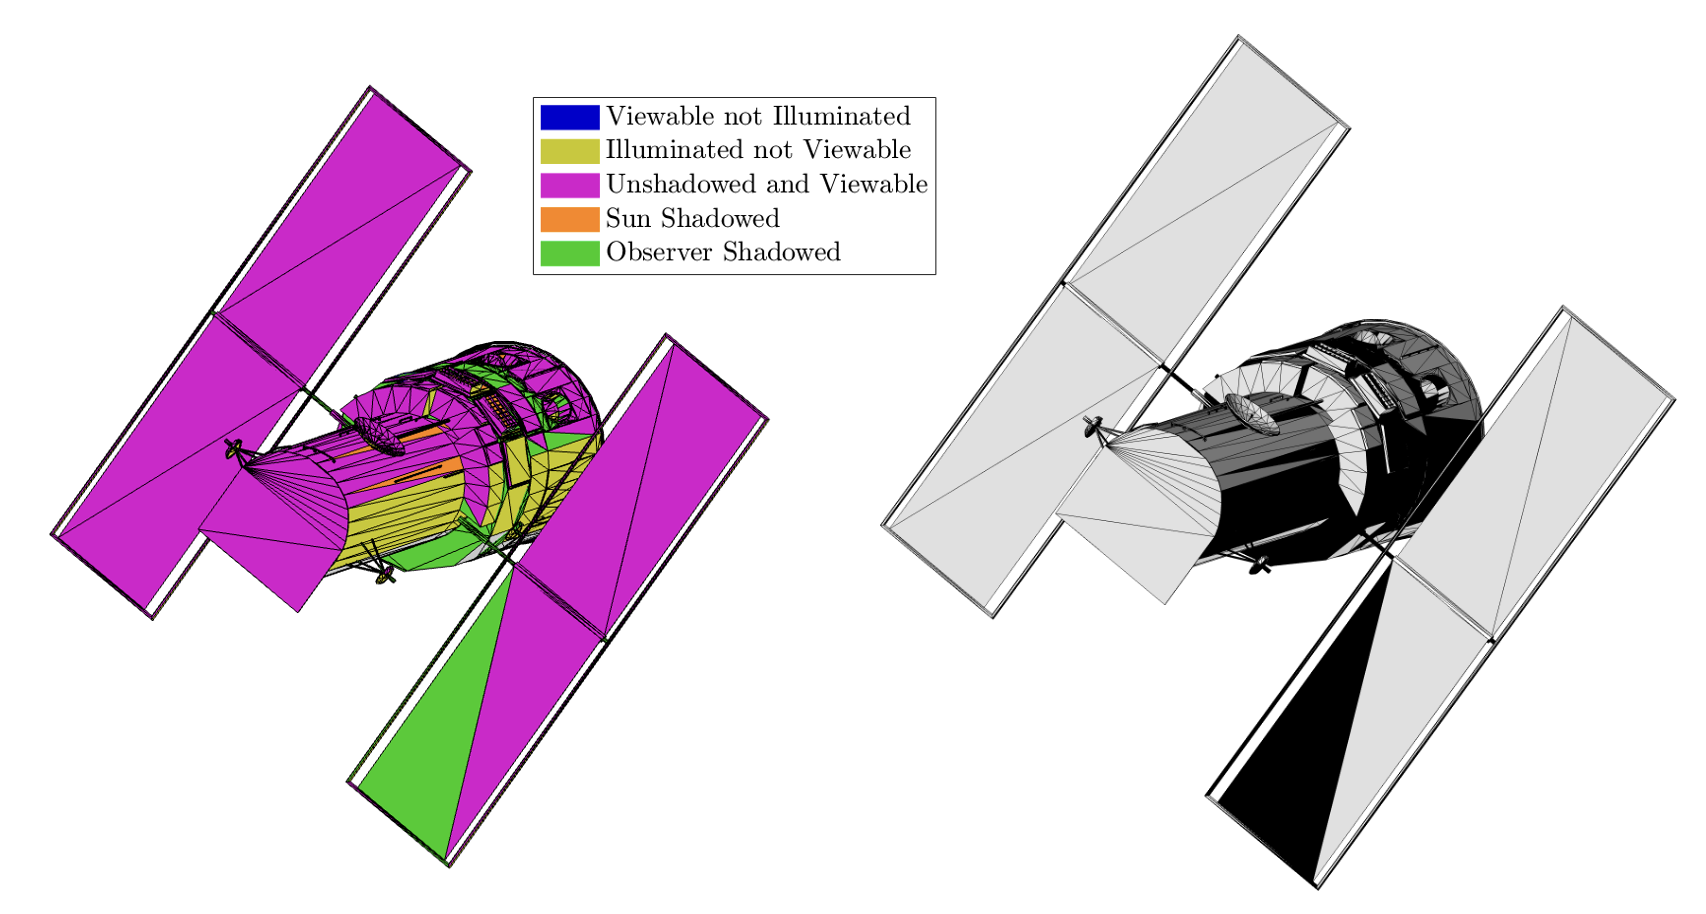
\includegraphics[width=350px]{hst_shadow_mapping/composite_hst_raytraced.png}
  \caption{Hubble Space Telescope ray traced shadow categorization and shading. Models from \cite{nasa_models}}
  \label{fig:hst_shadows_ray}
\end{figure}

The facet-wise shadow categorization shown in Figure \ref{fig:hst_shadows_ray} informs the $\mu_{ij}$ self-shadowing term in Eq \ref{eq:lc_func_normalized}. The major downside of facet-wise shadow categorization is that it is difficult to determine the fraction of each face is illuminated --- it categorizes the entire face together, leading to unphysical discontinuities in simulated light curves.

\subsubsection{The Importance of Self-Shadowing}

To motivate the need for accurate shadows when dealing with human-made space objects, consider the error introduced by neglecting shadows for different types of space objects. Kaasalainen and Torppa's work on asteroids reasonably assumed that shadowing was a negligible contribution to the measured light curve. Human-made objects do not afford the same luxury. Figure \ref{fig:hst_bennu_shadows} displays light curves for the asteroid Bennu and the Hubble Space Telescope with and without accurate shadows under a single-axis spin profile with inertially fixed Sun and observer vectors. Without accurate shadowing, the light curve's intensity and its time derivative can be significantly error-prone.

\begin{figure}[!htb]
  \centering
  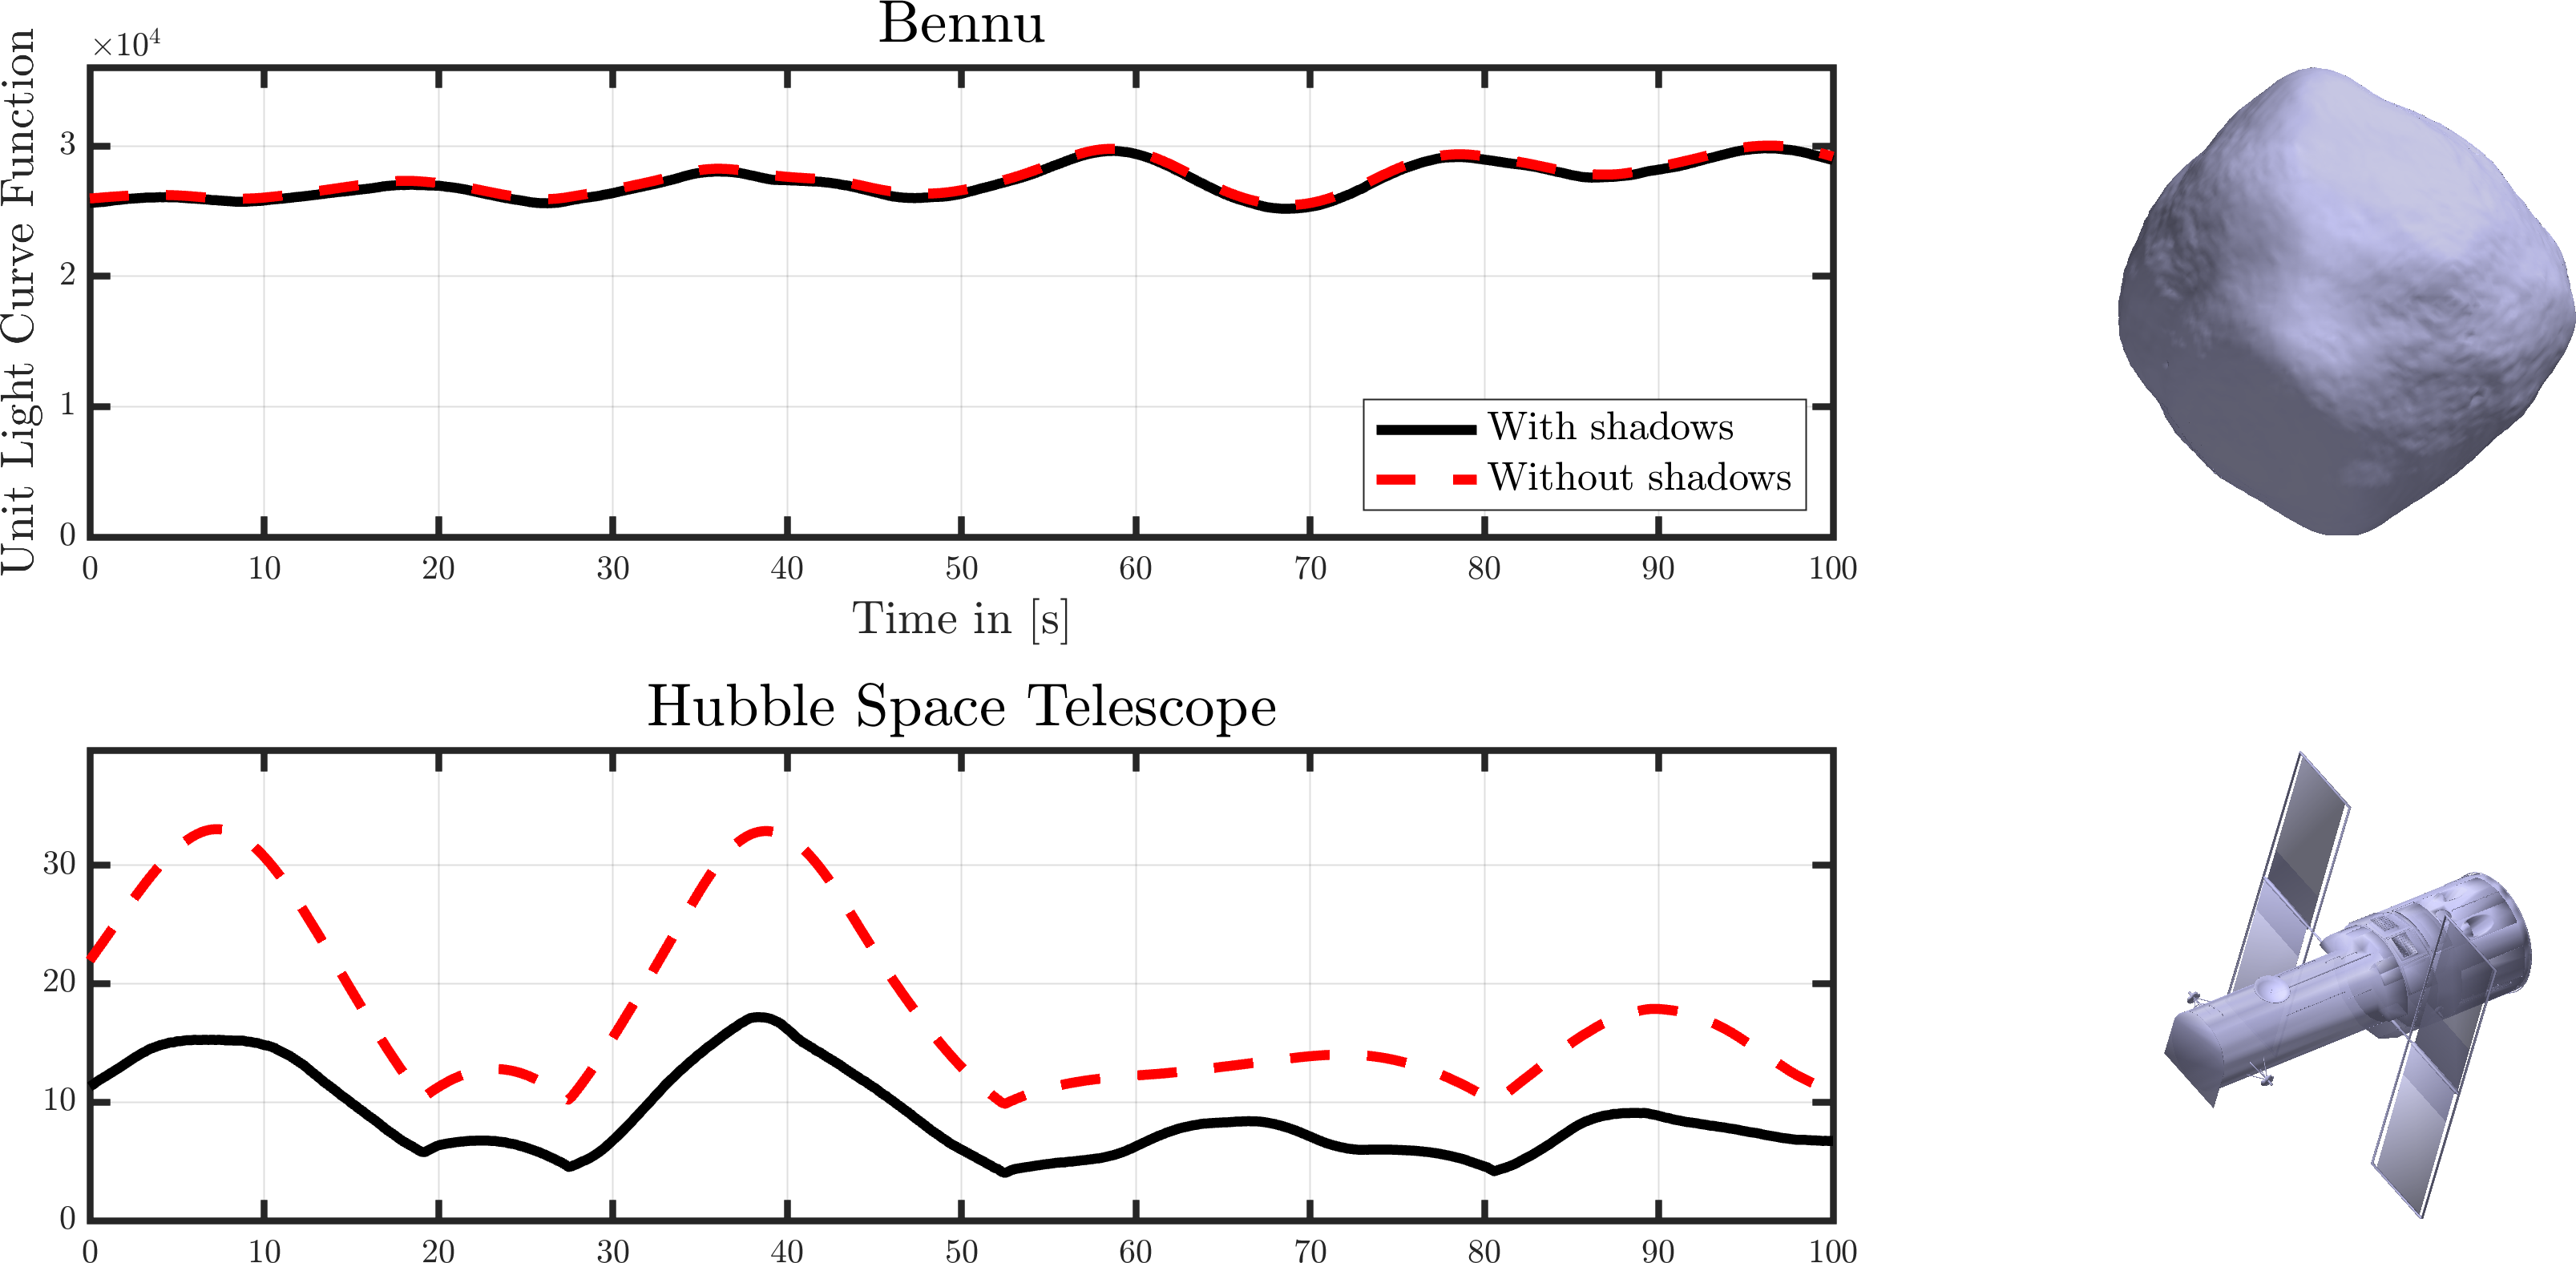
\includegraphics[width=350px]{convex_vs_nconv_lcs.png}
  \caption{Normalized irradiance errors introduced by neglecting shadows for Bennu and HST. Models from \cite{nasa_models}}
  \label{fig:hst_bennu_shadows}
\end{figure}

\subsubsection{Shadow Mapping} \label{sec:shadow_mapping}

Shadow mapping is used in the simulations presented in this work for faster and more accurate self-shadowing. Shadow mapping is a well understood technique in computer graphics \cite{kolivand2013}. Although modern ray traced shadowing may be more computationally efficient, shadow mapping was selected for its ease of implementation \cite{kolivand2013}. Shadow mapping shades individual pixel fragments instead of entire faces, offering increasing shadow quality over facewise ray tracing as the number of mesh faces falls.

Given an observer and Sun vector in the body frame of the object, shadow mapping proceeds in a four step process. In step one, a camera is positioned along the Sun vector and a perpendicular depth texture is computed. In the second step, depth values in Sun camera space are transformed to observer camera space, where a second depth texture is computed. This second texture is used to find the closest fragment along each ray to the Sun \cite{brabec2002}. Self-shadowed fragments are classified as those further from the Sun than the closest fragment along the same ray, indicated in red in Figure \ref{fig:hst_shadows_map}. Fragments that do not pass the convex shadowing condition are horizon shadowed, indicated in blue in Figure \ref{fig:hst_shadows_map}, determining the Sun and observer shadowing conditions at once. All remaining fragments are shaded with using the same Lambertian reflection model in \ref{eq:lc_func_normalized}. Computing the light curve function for the final rendered image requires summing all pixel values and dimensionalizing the result by the area of the observer camera's field of view. The light curve simulation environment used in this work was implemented in C and OpenGL \cite{raylib}.

In order to compute the final shaded and shadowed image, a depth map must be computed from the perspective of two orthographic cameras in the Sun and observer directions. These depth masks require a set of transformations from the model body frame to screen space. With this background laid out, the process for computing a perpendicular depth map $d(x,y)$ from the perspective of an arbitrary orthographic camera is detailed in Algorithm \ref{alg:depth_map}.

\begin{algorithm}
  \caption{Pixel-wise depth map computation for shadow mapping} \label{alg:depth_map}
  \begin{algorithmic}
    \State $(x, y) \in \mathbb{Z}$ \Comment{Pixel coordinates on the image plane}
    \State $\vctr{R}_\mathrm{pix} \in \mathbb{R}^3$ \Comment{Pixel world coordinates; provided by OpenGL}
    \State $d(x, y) \gets \left( \vctr{R}_{cam} - \vctr{R}_\mathrm{pix} \right) \cdot \vctr{R}_{cam}$ \Comment{Pixel depth in the camera view direction}
  \end{algorithmic}
\end{algorithm}

The pixel-wise shading process is summarized in Algorithm \ref{alg:pix_shading} in Appendix \ref{data:shading}. This shading and shadow mapping procedure is detailed graphically in Figure \ref{fig:hst_shadows_map}.

\begin{figure}[!htb]
  \centering
  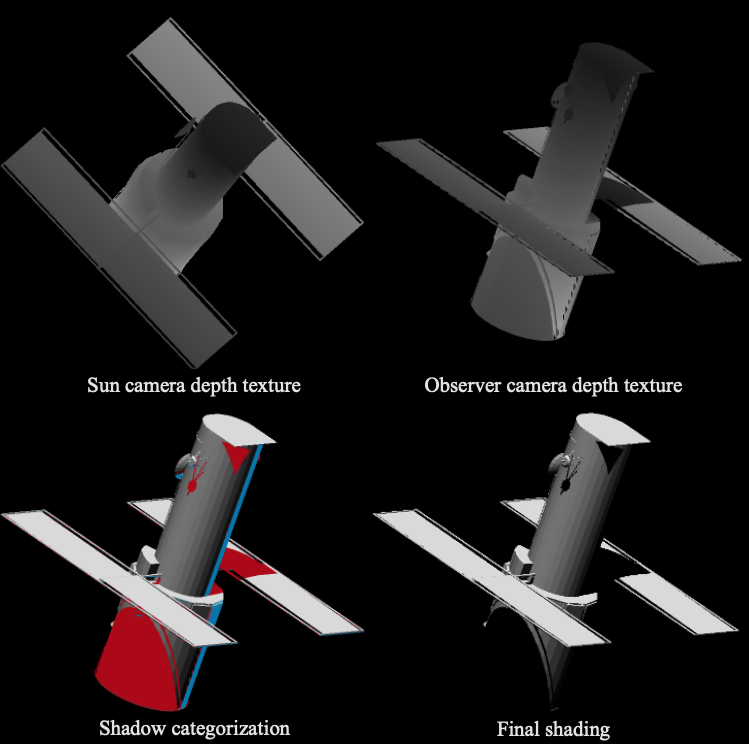
\includegraphics[width=\figmed]{hst_shadow_mapping/hst_shadow_mapping.png}
  \caption{Hubble Space Telescope shadow mapping with self (red) and horizon (blue) shadows rendered. Models from \cite{nasa_models}}
  \label{fig:hst_shadows_map}
\end{figure}
\graphicspath{{/Users/liamrobinson/Documents/PyLightCurves/docs/build/html/_images}}

An image shaded by Algorithm \ref{alg:pix_shading} is dimensionalized to a normalized irradiance value by computing the area of the square orthographic field of view given the image pixel count $n_\mathrm{pix}$:

\begin{equation} \label{eq:ortho_area}
  A_{image} = 2 n_\mathrm{pix} \left(FOV \right)^2.
\end{equation}

This field of view must be set dynamically at runtime to account for the size of the 3D model. The pixel values $v$ in the image are stored as unsigned 8 bit integers which take on values from 0 to 255, corresponding to the power range 0 to 1 within the pixel shading procedure described by Algorithm \ref{alg:pix_shading}. The total normalized irradiance in image $j$ is computed by summing over all $n_\mathrm{pix}$ pixels and dimensionalizing by the area of the image plane:

\begin{equation} \label{eq:lc_normalized_engine}
  \check{I}_j = \frac{A_{image}}{n_\mathrm{pix}} \sum_{i=1}^{n_\mathrm{pix}}{\frac{v_{i}}{255}}
\end{equation}

\section{Simulating The Observations}

\section{Time Systems}

In order to accurately predict the position of a space object and an observer, it is necessary to understand how a given time translates to the orientation of the relevant reference frames. These calculations require conversions between various time scales, the Julian date, and sidereal time.

\subsection{Time Scales}

There are a variety of scales used to measure time. What follows is a minimal treatment of each. For a more comprehensive overview, see Section 3.5 of \cite{vallado4ed}. International Atomic Time (TAI) is based on measurements from atomic clocks and is independent of astronomical effects or observations. By definition, TAI proceeds at the rate of $1$ SI second per second. Universal Time (UT0) is derived directly from observations of the apparent position of the stars. UT1 is derived from UT0 by adjusting for polar motion. UT1 is offset from TAI by $\Delta UT1$, which is a dynamic quantity that must be continually observed. Universal Coordinated Time (UTC) is a truncation of UT1 that uses an integer number of leap seconds $\Delta AT$ to stay within $0.9$ seconds of TAI. Terrestrial Time (TT) is defined by a constant offset of $TT - TAI = 32.184$ seconds from TAI and preceding at the same rate as TAI. These time scale relations are summarized in Eq \ref{eq:time_scale_conversions}.

\begin{align*}  \label{eq:time_scale_conversions} \numberthis
  UTC &= UT1 - \Delta UT1 \\
  TAI &= UTC + \Delta AT \\
  TT &= TAI + 32.184^s \\
\end{align*}

These time scales are relevant for this research as the precise coordinate frame transformation from ITRF to the J2000.0 realization of ICRF relies on quantities expressed in UT1. Date timestamps are usually standardized to UTC, requiring the transformations in Eq \ref{eq:time_scale_conversions} for full accuracy. Figure \ref{fig:time_scales} shows the evolution of UTC, UT1, and TT with respect to TAI. Notice that $\Delta UT1$ continually changes while $\Delta AT$ is always truncated to a nearby integer.

\begin{figure}[ht]
  \centering
  \includegraphics[width=\figbig]{sphx_glr_time_systems_001.png}
  \caption{Time scales relative to TAI}
  \label{fig:time_scales}
\end{figure}

\subsection{Julian Date}

Most tasks in astrodynamics are easier when using a continuous time system. For this reason, the Julian date is adopted. This quantity is defined as the number of days elapsed since January 1, 4713 B.C., at 12:00 \cite{vallado4ed}. Given a date timestamp of the form D/M/Y h:m:s between the years of 1900 and 2100, the Julian date is computed via:

\begin{equation} \label{eq:date_to_jd}
  JD = 376Y - \fl{\left[ \frac{7Y + 7 \cdot \fl{\left(\frac{M + 9}{12} \right)}}{4} \right]}
      + \fl{\left(\frac{275M}{9}\right)} 
      + d
      + 1721013.5
      + \frac{\frac{\left(\frac{s}{60} + 60\right)}{60} + h}{24}.
\end{equation}

Note that Eq \ref{eq:date_to_jd} is always a function of the time scale used in the input, i.\,e.\, a UTC timestamp yields $JD_{UTC}$ whereas a UT1 timestamp yields $JD_{UT1}$. Another useful quantity for later time and coordinate system calculations is the number of Julian centuries since a particular epoch. The J2000.0 epoch is used unless otherwise stated, resulting in \cite{vallado4ed}:

\begin{equation} \label{eq:jd_to_t}
  T = \frac{JD - 2451545.0}{36535}.
\end{equation}

Often, more specificity is needed with respect to the time scale used in Eq \ref{eq:jd_to_t}. For example, computing $T$ with an input date in UT1 yields $T_{UT1}$ using $JD_{UT1}$, which is in turn a function of a date expressed in UT1. 

\subsection{Solar and Sidereal Time}

A solar day is defined as the time required for the Sun to pass and return to an observer's meridian --- a line of constant longitude extending from the geographic south pole to the geographic north pole \cite{vallado4ed}. By contrast, a sidereal day is the time required for the stars to complete a revolution around an observer's meridian. Due to the Earth's orbit around the Sun, the sidereal day is about 4 minutes shorter than the solar day \cite{vallado4ed}. The Greenwich mean sidereal time (GMST) is computed in seconds via \cite{frueh2019notes}:

\begin{equation} \label{eq:date_to_gmst}
  \theta_{GMST} = 67310.54841
        + \left(3.15576 \cdot 10^9 + 8640184.812866 \right) T_{UT1}
        + 0.093104 T_{UT1}^2
        - 6.2 \cdot 10^{-6} T_{UT1}^3.
\end{equation}

Accounting for the variations in the inclination of the ecliptic $\epsilon$ and the change in the equinox compared to the reference epoch $\Delta \Psi$ produces Greenwich apparent sidereal time (GAST) via \cite{frueh2019notes}:

\begin{equation} \label{eq:date_to_gast}
  \theta_{GAST} = \theta_{GMST} + \Delta \Psi \cos\epsilon.
\end{equation}

Both the inclination of the ecliptic and the difference in the equinox are computed with series expansions following the IAU 1980 theory of nutation \cite{vallado4ed}.

\section{Coordinate Systems}

A precise definition of coordinate systems is necessary for determining the position of the observer and the observed space object at a given time. The relevant conversions are summarized by a single question: how is a fixed position on the surface of the Earth transformed into a standardized inertial reference frame?

\subsection{Latitude, Longitude and Altitude}

Latitude, longitude, and altitude (LLA) is a spherical representation of position on or above the surface of the Earth. For the purposes of precise station positioning, the difference between the two types of longitude --- geocentric and geodetic --- is important. Geocentric latitude is the angle between the line from the center of mass of the Earth to the position of interest and the equatorial plane. Geodetic latitude instead measures the angle between the local ellipsoid surface normal and the equatorial plane. Geodetic latitude $\phi_\mathrm{geod}$ is converted to geocentric $\phi_\mathrm{geoc}$ latitude with \cite{frueh2019notes}:

\begin{equation} \label{eq:geod_to_geoc}
  \phi_\mathrm{geoc} = \tan^{-1} \left((1 - f)^2 \tan\phi_\mathrm{geod} \right).
\end{equation}

Additionally, the radius of the ellipsoid $r_E$ at a given geocentric latitude is necessary for later conversion, expressed by \cite{frueh2019notes}:

\begin{equation} \label{eq:rad_at_geoc}
  r_E = R_E - f \sin^2 \left( \phi_\mathrm{geoc} \right).
\end{equation}

The altitude in a set of LLA coordinates needs a reference point. Different observers may be defined differently --- either relative to the approximate ellipsoidal shape of the Earth, the hypothetical mean sea level, or the surrounding terrain.

\subsubsection{Ellipsoid}

Due to Earth's equatorial bulge, it is common to model the rough shape of the Earth as an ellipsoid. In particular, the 1984 World Geodetic Survey (WGS-84) model is used throughout this work to define the shape of the Earth ellipsoid, with parameters listed in Table \ref{tb:wgs84} for use in Eqs \ref{eq:geod_to_geoc} and \ref{eq:rad_at_geoc}.

\begin{table}[ht]
  \centering
  \begin{tabular}{|l|l|}
  \hline
  \textbf{Parameter} & \textbf{Value}              \\ \hline
  Equatorial radius $R_E$             & $6378.137 \: [km]$ \\ \hline
  Flattening ratio $f$                & $1 / 298.257$      \\ \hline
  \end{tabular}
  \caption{WGS-84 ellipsoid model of the Earth \cite{vallado4ed}.}
  \label{tb:wgs84}
\end{table}

These parameters are needed for the conversion from LLA to the International Terrestrial Reference Frame.

\subsubsection{Geoid}

The geoid accounts for the gravitational potential differences across the Earth's surface \cite{vallado4ed}. It is a surface of equal gravitational potential; the surface the ocean relaxes to without the influence of the wind and tides \cite{vallado4ed}. For this reason, the geoid is alternatively known as the mean sea level (MSL). The ellipsoid is a good approximation of the geoid, which deviates from the ellipsoid by less than $\approx 100$ meters at all latitudes and longitudes. The height of the geoid above the ellipsoid can be computed from a high-fidelity gravity model, but it is often more convenient to interpolate a pre-computed grid of geoid heights. Figure \ref{fig:geoid_shape} displays global geoid heights derived from the 1996 Earth Gravitational Model (EGM-96) relative to the ellipsoid.

\begin{figure}[ht]
  \centering
  \includegraphics[width=\figbig]{sphx_glr_geoid_heights_001_2_00x.png}
  \caption{EGM-96 geoid heights above the WGS-84 ellipsoid}
  \label{fig:geoid_shape}
\end{figure}

\subsubsection{Terrain}

Terrain elevation is usually the final component needed to fully define the altitude of a ground station, which is often defined relative to MSL. This work uses $30$-meter terrain tiles from the Shuttle Radar Topography Mission (SRTM). Figure \ref{fig:pogs_terrain} shows the local elevation around the Purdue Optical Ground Station using SRTM data.

\begin{figure}[ht]
  \centering
  \includegraphics[width=\figmed]{sphx_glr_pogs_local_terrain_001.png}
  \caption{MSL elevations surrounding the Purdue Optical Ground Station}
  \label{fig:pogs_terrain}
\end{figure}

\subsubsection{Altitude Conversions}

Given an altitude relative to the terrain $a_\mathrm{terrain}$, the elevation above the ellipsoid $a_\mathrm{ellip}$ is given as a function of the terrain elevation above the geoid $h_\mathrm{terrain}(\lambda, \phi)$ and the geoid elevation above the ellipsoid $h_\mathrm{terrain}(\lambda, \phi)$ by \cite{vallado4ed}:

\begin{equation} \label{eq:altitude_above_ellipsoid}
  a_\mathrm{ellip} = a_\mathrm{terrain} + h_\mathrm{terrain}(\lambda, \phi_\mathrm{geod}) + h_\mathrm{geoid}(\lambda, \phi_\mathrm{geod}).
\end{equation}

\subsection{International Terrestrial Reference Frame (ITRF)}

The Cartesian form of LLA is known as the Earth-centered Earth-fixed (ECEF) reference frame. Throughout this work, ECEF and ITRF will be used interchangeably. This frame has its origin at the center of mass of the Earth and its axes fixed in the crust. The
fundamental plane of the frame is defined to be the equator ---  orienting the $z$-axis through Earth's
instantaneous spin axis, and the reference direction through the intersection of the prime meridian
and the equator ---  defining the $x$-axis. Completing the right-handed system with $\hat{y} = \hat{z} \times \hat{x}$ yields a
reference frame that remains fixed, neglecting effects like continental drift. The transformation from LLA $\left( \lambda, \phi_\mathrm{geod}, a_\mathrm{ellip} \right)$ to ITRF is given by \cite{vallado4ed}:

\begin{align*} \numberthis \label{eq:lla_to_itrf}
  e^2 &= 2f - f^2 \\
  N &= \frac{R_E}{\sqrt(1 - e^2 \sin(\phi_\mathrm{geod})^2)} \\
  \rho &= (N + a_{\mathrm{ellip}}) \cos(\phi_\mathrm{geod}) \\
  x_\mathrm{itrf} &= \rho \cos(\lambda) \\
  y_\mathrm{itrf} &= \rho \sin(\lambda) \\
  z_\mathrm{itrf} &= \left(N (1 - e^2) + a_{\mathrm{ellip}} \right) \sin(\phi_\mathrm{geod}). \\
\end{align*}

In Eq \ref{eq:lla_to_itrf}, $e^2$ is the squared eccentricity of the ellipsoid, $N$ is the radius of curvature in the meridian, and $\rho$ is the $x-y$ plane magnitude of the station's position \cite{vallado4ed}.

Many later transformations require the body axis rotation matrices $R_1$, $R_2$, and $R_3$ which are expressed:

\begin{align*} \numberthis \label{eq:body_rotms}
  R_1(\theta) &= \begin{bmatrix}  1 & 0 & 0 \\ 0 & \cos\theta & \sin\theta \\ 0 & -\sin\theta & \cos\theta \end{bmatrix} \\
  R_2(\theta) &= \begin{bmatrix}  \cos\theta & 0 & -\sin\theta \\ 0 & 1 & 0 \\ \sin\theta & 0 & \cos\theta \end{bmatrix} \\
  R_3(\theta) &= \begin{bmatrix}  \cos\theta & \sin\theta & 0 \\ -\sin\theta & \cos\theta & 0 \\ 0 & 0 & 1 \end{bmatrix}. \\
\end{align*}

\subsection{Topocentric East North Up (ENU) Reference Frame}

The remaining transformations in this chapter will only be defined in terms of their rotation matrices. It is often useful to express observations in a local reference frame. The East North Up (ENU) coordinate system is used throughout this work. This system has an origin at the observing station, with the first two basis vectors pointing towards the local East and North and the third pointing towards zenith. The transformation from a vector $\vctr{r}_\mathrm{itrf}$ in ITRF to $\vctr{r}_{enu}$ in ENU is a function of the longitude of the station $\lambda$ and the geocentric latitude $\phi_\mathrm{geoc}$ by \cite{frueh2019notes}:

\begin{equation} \label{eq:itrf_to_enu}
  \vctr{r}_{enu} = F_2 F_1 R_2(\phi_\mathrm{geoc}) R_3(\lambda) \vctr{r}_\mathrm{itrf}.
\end{equation}

In Eq \ref{eq:itrf_to_enu}, $R_3$ is a rotation about the third body axis, $F_1$ swaps the second and third unit vectors, and $F_2$ swaps the first and third unit vectors. The orientation of the ENU reference frame at the Purdue Optical Ground Station is depicted in Figure \ref{fig:pogs_enu}.

\begin{figure}[ht]
  \centering
  \includegraphics[width=\figmed]{sphx_glr_az_el_parallel_001.png}
  \caption{ENU reference frame orientation at Purdue Optical Ground Station}
  \label{fig:pogs_enu}
\end{figure}

\subsection{International Celestial Reference Frame (ICRF/J2000)} \label{sec:teme}

Transforming from ITRF to a standardized inertial reference frame is an involved process due to the variety of nonlinear effects impacting the Earth's rotational motion. In total, this transformation must account for polar motion, the nutation and precession of the Earth's pole, and the mean sidereal time. These transformations are treated much more thoroughly in Montenbruck and Gill \cite{montenbruck2012}. 

Accounting for polar motion --- the motion of the Earth's pole that cannot be explained through nutation theory --- transforms from $\vctr{r}_\mathrm{itrf}$ in ITRF to $\vctr{r}_{gtod}$ in Greenwich True of Date (GTOD) via \cite{vallado4ed}:

\begin{equation} \label{eq:itrf_to_gtod}
  \vctr{r}_{gtod} = R_1(y_p) R_2(x_p) \vctr{r}_\mathrm{itrf},
\end{equation}

where $x_p$ and $y_p$ are the angular components of the polar motion at the time of interest \cite{frueh2019notes}. Accounting for the sidereal rotation of the Earth about its pole transforms from $\vctr{r}_{gtod}$ in GTOD to $\vctr{r}_{teme}$ in the True Equator, Mean Equinox (TEME) reference frame via \cite{frueh2019notes}:

\begin{equation} \label{eq:gtod_to_teme}
  \vctr{r}_{teme} = R_3(-\theta_{GMST}) \vctr{r}_{gtod},
\end{equation}

where $\theta_{GMST}$ is the Greenwich mean sidereal time. Accounting for the difference between GMST and GAST at the date of interest transforms $\vctr{r}_{teme}$ TEME to $\vctr{r}_{tod}$ in the True of Date (TOD) reference frame via \cite{vallado4ed}:

\begin{equation} \label{eq:teme_to_tod}
  \vctr{r}_{tod} = R_3(-\Delta \Psi \cos \epsilon) \vctr{r}_{teme},
\end{equation}

where $\Delta \Psi$ is the angular difference in the longitude of the vernal equinox between GMST and GAST, and $\epsilon$ is the true inclination of the ecliptic \cite{vallado4ed}. Accounting for the nutation of Earth's pole transforms $\vctr{r}_{tod}$ from TOD to $\vctr{r}_{mod}$ in the Mean of Date (MOD) reference frame via \cite{vallado4ed}:

\begin{equation} \label{eq:tod_to_mod}
  \vctr{r}_{mod} = R_1(-\bar{\epsilon}) R_3(\Delta\Psi) R_1(\bar{\epsilon} + \Delta\epsilon) \vctr{r}_{tod},
\end{equation}

where $\bar{\epsilon}$ is the mean inclination of the ecliptic at the time of interest, and $\epsilon$ is the true inclination of the ecliptic \cite{vallado4ed}.

Accounting for the secular precession of Earth's pole transforms $\vctr{r}_{mod}$ from MOD to $\vctr{r}_\mathrm{icrf}$ in ICRF via \cite{vallado4ed}:

\begin{equation} \label{eq:mod_to_icrf}
  \vctr{r}_\mathrm{icrf} = R_3(\zeta) R_2(\theta) R_3(z) \vctr{r}_{mod},
\end{equation}

through the 3-2-3 Euler angle sequence $\left( z, \theta, \zeta \right)$. Each of these angles modeling the precession are a function of the date of the transformation, and are approximated by polynomial expansions in the Julian century $T$ \cite{frueh2019notes}.

The specific realization of ICRF used in this work is referenced to the position of the equator and equinox at the J2000.0 epoch (January 1, 2000 12:00:00.000 TT), leading to the common name for this reference frame, "J2000" \cite{vallado4ed}.

\subsection{Right Ascension and Declination}

Right ascension and declination, often shortened to RA/Dec, are useful angles for describing the angular position of an object on the celestial sphere from the perspective of an observer. As such, RA/Dec values are inertial, but can be defined relative to a topocentric observer or the center of the Earth \cite{frueh2019notes}. The topocentric RA/Dec is exclusively used in this work for later simulations. Right ascension is defined as the angle
of the observation projected onto the inertial $x-y$ plane, measured counterclockwise from inertial
$\hat{x}$, represented by $\alpha$. Declination is the angle from the $x-y$ plane to the observation
with positive values above the $x-y$ plane (closer to inertial $z$) and negative values below.
Declination is represented by $\delta$. Given a unit vector direction $\hat{v} = \left[ x_\mathrm{itrf}, y_\mathrm{itrf}, z_\mathrm{itrf} \right]^T$ in J2000, RA/Dec is computed via \cite{frueh2019notes}:

\begin{equation} \label{eq:eci_to_ra_dec}
  \begin{bmatrix}
	\alpha \\
	\delta
  \end{bmatrix} = 
  \begin{bmatrix}
	\atantwo(y_\mathrm{itrf}, x_\mathrm{itrf}) \\
	\atantwo(z_\mathrm{itrf}, \sqrt{x_\mathrm{itrf}^2 + y_\mathrm{itrf}^2})
  \end{bmatrix}.
\end{equation}

\subsection{Azimuth and Elevation}

Azimuth and elevation, often shortened to Az/El, are similar angular quantities to right ascension and declination \cite{frueh2019notes}. Instead of being based on
the inertial sphere, they are referenced to an arbitrary reference frame. For a telescope making
observations of an object, the local topocentric ENU frame may be used. For a satellite star
tracker, star azimuth and elevation might be reported in the satellite body frame. In either case,
Eq \ref{eq:eci_to_ra_dec} can be repurposed in terms of Az/El, where $\hat{v} = \left[ x_{ENU}, y_{ENU}, z_{ENU}
\right]^T$ is expressed in the frame of interest \cite{frueh2019notes}.

\begin{equation} \label{eq:enu_to_az_el}
  \begin{bmatrix}
	Az \\
	El
  \end{bmatrix} = 
  \begin{bmatrix}
	\atantwo(y_{ENU}, x_{ENU}) \\
	\atantwo(z_{ENU}, \sqrt{x_{ENU}^2 + y_{ENU}^2})
  \end{bmatrix}
\end{equation}

Note that Eq \ref{eq:enu_to_az_el} references azimuth to the $x$-axis, proceeding in the
counterclockwise direction. Often, this reference axis and direction may be changed depending on the
reference frame being used. For example, ground station observations may be referenced to local
North ---  the second axis of the ENU system ---  proceeding clockwise. This would require the
substitution $Az' = \frac{\pi}{2} - Az$. Notice that this substitution leads to $Az'$ leaking
outside the domain of $[0, 2\pi)$. This is not an issue for later coordinate transformations but
may be undesirable for plots. Wrapping the result back to the standard azimuth range via
$Az_{wrapped} = \textrm{mod}(Az, 2\pi)$ is a sufficient fix.

\subsection{Coordinate Transformations Summary}

With these transformations, any topocentric observation directions in RA/Dec or Az/El can be converted into a Cartesian representation and transformed into J2000. Simultaneously, any propagated space object orbits can be transformed similarly from an arbitrary propagation frame such that all future computations requiring the observation geometry take place in the same reference frame. 

\subsection{Planetary Ephemerides} \label{sec:planet_ephem}

The Spacecraft, Planet, Instrument, C-matrix, and Events (SPICE) toolkit is used for the propagation of the Sun and Moon throughout the results presented in this work \cite{spice}. SPICE is maintained by the NASA Jet Propulsion Laboratory's Navigation and Ancillary Information Facility (NAIF) and provides the state of the art solutions for the positions and orientations of solar system bodies \cite{spice}. All calculations of $\vctr{r}_{Sun}$ and $\vctr{r}_\mathrm{Moon}$ rely on queries to SPICE using the DE440s planetary ephemeris files.

\section{The Charge Coupled Device (CCD)} \label{sec:ccd_performance}

Many optical telescopes, including the Purdue Optical Ground Station, use a CCD to convert incident photons into a digital signal on a pixel grid \cite{krag2003}. CCDs accomplish this with a matrix of semiconductor pixel wells which collect electrons released by the photoelectric effect when photons are incident on that pixel \cite{krag2003}. The release of these photoelectrons is wavelength dependent and is captured by the quantum efficiency spectrum of a given CCD. Developing this background in photometry is useful for both light curve simulation as well as simulating the CCD camera measuring that light curve. 

Due to the sheer distance from the observer to any space object, taking an image that resolves the object's geometry is generally impossible. For an observer with the pixel scale of the Purdue Optical Ground Station ($s_\mathrm{pix} = 0.72 \: [arcsec/pixel]$), a 6U CubeSat in LEO occupies about 1/44 of a pixel area, while a large communications satellite in GEO occupies approximately 1/13 of a pixel area. In either case, no geometric information is left on the image plane even before diffraction is taken into account. 

Whenever an optical telescope is observing an unresolved space object, the object's signal is necessarily superimposed on whatever signals exist in the background as the unresolved signal spreads much farther than the object's actual geometric bounds. In this context, background does not only refer to sources physically further than the object --- as light can easily enter optical path through atmospheric scattering --- but all sources that impact the image apart from the object signal. Some of these sources even originate within the telescope optics and its sensor. To faithfully simulate a telescope observing an object, many position-based SDA tasks are able to ignore background effects while acquiring or tracking objects. For photometry-based SDA, the background is critical. The overall noise floor can be broken up into background signal sources and sensor effects.

\subsection{Diffraction}

Many objects of interest are far past LEO, making optical observations diffraction limited. Diffraction is always occurring when observing an object at any distance through any optics, but it begins to dominate when the object's scale is equal or smaller than the Rayleigh criterion \cite{frueh2019notes}.

\subsubsection{Rayleigh Criterion}

The Rayleigh criterion states that light of wavelength $\lambda$ will spread into a diffraction pattern with the first minimum of the distribution at an angular radius $\theta_R$ when passing through a circular aperture of diameter $d$ \cite{frueh2019notes} such that:

\begin{align*} \numberthis \label{eq:rayleigh_criterion}
  \sin\theta_R &= \frac{1.22 \lambda}{d}, \\
  \theta_R &\approx \frac{1.22 \lambda}{d}.
\end{align*}

For a $0.5$-meter aperture optical telescope with a pixel scale of $1$ arcsecond per pixel, observing a $40$-meter wide object in GEO --- occupying approximately $0.2$ pixel widths on the image --- Eq \ref{eq:rayleigh_criterion} predicts that the diffraction pattern will be $2.4$ times wider than the object at a wavelength of $550$ nanometers. Similarly, a $60$-centimeter wide object in LEO observed with the same telescope occupies $0.1$ pixel widths in the image while producing an Airy disk $4.5$ times wider than the object itself. As a result, GEO objects cannot be resolved from the ground, independent of atmospheric effects. 

\subsubsection{The Airy Disk}

The far-field diffraction pattern produced by a point source is known as an Airy pattern or disk \cite{frueh2019notes}. The Airy disk is expressed in terms of an amplitude $C$ at an angular distance $\theta$ from the center $C(\theta)$ \cite{frueh2019notes} as:

\begin{equation} \label{eq:airy_disk}
  C_{Airy}(\theta) = C_0 \left( \frac{2 J_1(k \cdot r_d \sin\theta)}{k \cdot r_d \sin\theta} \right).
\end{equation}

In Eq \ref{eq:airy_disk}, $C_0$ is the amplitude of the center of the Airy disk, $r_d$ is the radius of the aperture, $k = \frac{2\pi}{\lambda}$ is the wavenumber, and $J_1$ is the first order Bessel function of the first kind. The central magnitude $C_0$ is expressed:

\begin{equation} \label{eq:airy_center}
  C_0 = \frac{S_\mathrm{obj}^2 A_\mathrm{aperture}^2}{2 f^4}.
\end{equation}

In Eq \ref{eq:airy_center}, $S_\mathrm{obj}$ is the total mean irradiance incident on the CCD due to the source, $A_\mathrm{aperture}$ is the aperture area, and $f$ is the focal length of the optics \cite{frueh2019notes}. The pattern produced by Eq \ref{eq:airy_disk} is depicted in Figure \ref{fig:airy_disk_magnitude}.

\begin{figure}[ht]
  \centering
  \includegraphics[width=\figmed]{sphx_glr_airy_disk_diffraction_001_2_00x.png}
  \caption{Airy disk diffraction pattern}
  \label{fig:airy_disk_magnitude}
\end{figure}

The Rayleigh criterion expresses the angular size of the first zero of the Airy disk, after which the amplitude of the Airy disk drops off exponentially. It is often useful to approximate the Airy disk with a 2D Gaussian. Given the total signal to be approximated, this Gaussian is fit with a single parameter --- the full width at half maximum (FWHM). The FWHM expresses the diameter at which the signal drops to half the magnitude of its central maximum \cite{frueh2019notes}. The FWHM of the Airy disk is expressed \cite{frueh2019notes}:

\begin{equation} \label{eq:fwhm_airy}
  FWHM_\mathrm{Airy} = \frac{1.028 \lambda}{2 r_d}.
\end{equation}

The diffraction pattern is not the only effect that spreads the unresolved signal over the pixel grid. Atmospheric turbulence contributes to further spreading and speckling of the signal \cite{frueh2019notes}. This effect --- known as the \textit{seeing} --- is encapsulated in $FWHM_{seeing}$ and is generally between $1$ and $3$ arcseconds \cite{frueh2019notes}. While the seeing and diffraction pattern FWHMs are additive, it is sufficient to take the larger value for simulation purposes \cite{frueh2019notes}. The standard deviation of the Gaussian approximation of the Airy disk is given by:

\begin{equation} \label{eq:airy_variance}
  \sigma = \frac{FWHM}{2 \sqrt{2 \ln{2}}}.
\end{equation}

The full Gaussian approximation at an angular distance $\theta$ from the source is given by:

\begin{equation} \label{eq:airy_gaussian}
  C_{Gauss}(\theta) = \frac{0.838 \bar{C}_\mathrm{all}}{2 \pi \sigma^2} \exp\left( - \frac{\theta^2}{2 \sigma^2} \right)
\end{equation}

In practice, computing the Airy disk or its Gaussian approximation on rectangular pixel grid amounts to integrating the amplitude function $C(\theta)$ over the pixel area:

\begin{equation} \label{eq:pix_values_gauss}
  C_\mathrm{pix}(x, y) = \int_{x}^{x + \Delta x} \int_{y}^{y + \Delta y}{C_{Gauss}(\theta(x, y))} \: dy \: dy.
\end{equation}

The area within the first maximum of the Airy disk is given by \cite{frueh2019notes}:

\begin{equation} \label{eq:airy_area}
  A_\mathrm{Airy} = \pi \left(\frac{648000 / \pi}{s_\mathrm{pix}} \sin^{-1}\left(\frac{1.22 \lambda}{D}\right) \right)^2.
\end{equation}

\subsection{Signal-to-Noise Ratio (SNR)}

Because the unresolved object signals are always superimposed on the background of the image, the SNR of a CCD is expressed with the signal included in the denominator noise term \cite{frueh2019notes}:

\begin{equation} \label{eq:ccd_snr}
  SNR = \frac{S_\mathrm{obj}}{\sqrt{S_\mathrm{obj}+N}}.
\end{equation}

Explicitly, the SNR can be expanded in terms of the signal means and variances, assuming that their respective probability density functions are independent \cite{frueh2019notes}:

\begin{equation} \label{eq:ccd_snr_expanded}
  SNR = \frac{S_\mathrm{obj}}{\sqrt{S_\mathrm{obj} + n_\mathrm{pix} \left( \lambda_\mathrm{background} + \lambda_{dark} + \sigma^2_\mathrm{read} + \frac{g^2}{24} \right)}}.
\end{equation}

It should be noted that the SNR computed in Eq \ref{eq:ccd_snr_expanded} is idealized. In reality, the discrete sampling of each random variable in each object pixel --- as well as the Poisson sampling of the object signal --- results in a slightly different value. As the number of object pixels approaches infinity, the SNR computed from the image would approach the theoretical value. Figure \ref{fig:snr_grid} illustrates the effect of raising the background noise level while holding the object signal constant on the SNR.

\begin{figure}[ht]
  \centering
  \includegraphics[width=\figmed]{sphx_glr_snr_001_2_00x.png}
  \caption{Signal-to-noise ratio reduction on a synthetic CCD pixel grid}
  \label{fig:snr_grid}
\end{figure}

The SNR is an important constraint when determining whether an object signal is visible above the background. If the SNR is too low, it becomes difficult or impossible to notice and quantify the object signal. Simulations in this work are all performed with a reasonable SNR limit of $3$.

\subsection{Telescope Properties} \label{sec:telescope_properties}

While much of the focus in this work is directed towards the CCD, the telescope it is mounted within has a few important properties which must be known for accurate CCD simulation. 

The aperture of the telescope is the beginning of the optical path within the telescope --- the area that collects incoming light. The area of the aperture $A_\mathrm{aperture} = \pi r_{d}^2$, where $r_d$ is the radius of the aperture must be distinguished from the \textit{effective} aperture area, which is the total area of the aperture which actually collects light. Some telescopes have central obstructions which remove an amount of aperture area from the optical path, such that the effective aperture area is:

\begin{equation}
  A_\mathrm{eff} = A_\mathrm{aperture} - \pi r_{o}^2,
\end{equation}

where $r_o$ is the radius of the obstruction. The telescope focal length $f$ is the length of the optical path within the optics required to resolve a focused image. The pixel scale $s_\mathrm{pix}$ is a measure of the angle spanned by the side length of each square pixel, often expressed in arcseconds per pixel. 

\subsection{Brightness Units}

In the context of photometry, "brightness" is a catch-all term for a variety of units. Defining the relationships between these units will make later light curve conversions more clear. Brightness conversions are needed for both light curves and the environmental data sources that drive the CCD performance model described in Section \ref{sec:ccd_performance}.

\subsubsection{$\mathbf{S_{10}}$ Surface Brightness}

While apparent magnitude and irradiance are effective for quantifying the flux of point sources, other units exist
to describe diffuse or extended sources where brightness is spread over an
area. $S_{10}$ is a unit of surface brightness representing the number of 10th magnitude stars per square degree that would produce the same flux as a given diffuse source.
Surface brightness in $S_{10}$ over a given solid angle $\Omega \: \left[ sr \right]$ can be converted to total irradiance $I \: \left[ \frac{W}{m^2} \right]$ via \cite{krag2003}:

\begin{equation} \label{eq:s10toirrad}
 \frac{I \left[ \frac{W}{m^2} \right]}{S_{10}} = 10^{-10/2.5} \left( \Omega \frac{180^2}{\pi^2} \right)
  \int_{10^{-8}}^{10^{-6}}{ \mathcal{ZM}(\lambda) \: d\lambda} = 8.26617 \Omega \cdot 10^{-9}.
\end{equation}

In \ref{eq:s10toirrad}, $\mathcal{ZM}(\lambda) \: \left[ \frac{W}{m^2 \cdot m} \right]$ is the
representative spectrum of a 0th magnitude star, $\textrm{QE}(\lambda)$ is the quantum efficiency
spectrum of the observing sensor, $\textrm{ATM}(\lambda)$ is the atmospheric transmission spectrum, $\lambda \: [m]$ is wavelength, $h \: \left[
\frac{m^2 \cdot kg}{s} \right]$ is Plank's constant, and $c \: \left[ \frac{m}{s^2} \right]$ is the
speed of light in vacuum. Quantum efficiency has units of photoelectrons, conveying the fraction of incident photons converted to photoelectrons in the CCD sensor. Atmospheric transmission is a unitless quantity conveying the fraction of light that is not absorbed by the atmosphere. Example spectra for $\textrm{ATM}(\lambda)$ and $\textrm{QE}(\lambda)$ are displayed in Figure \ref{fig:spectra}, with underlying data provided in Appendix \ref{data:atm}.

\subsubsection{Magnitude per Square Arcsecond}

A second surface brightness unit is $\left[ \frac{mag}{arcsec^2} \right]$, also known as MPSAS (magnitude per square arcsecond) \cite{krag2003}. This quantity can be thought of as a generalized $S_{10}$, where instead of quantifying the number of stars of a certain
magnitude in a solid angle, the equivalent magnitude of a single point source is measured. A surface
brightness $B_{10}$ in $S_{10}$ can be converted into surface brightness $B_{mag}$ in 
$\left[ \frac{mag}{arcsec^2} \right]$ by applying Eq \ref{eq:mag_to_irradiance}.

\begin{equation} \label{s10_to_mag_per_a2}
	B_{mag} = -2.5 \log_{10}\left( \frac{B_{10} \cdot 10^{-4}}{12960000} \right).
\end{equation}

In Eq \ref{s10_to_mag_per_a2} $B_{10}$ is converted to the total irradiance per square degree,
converted square degrees to square arcseconds, and finally transformed into apparent magnitude. $B_{mag}$ in MPSAS is converted to irradiance per steradian using \ref{eq:mag_to_irradiance}:

\begin{equation} \label{eq:mpsas_to_irrad_per_ster}
  I = \left( \frac{180}{ 3600\pi} \right)^2 I_s \cdot 10^{-\frac{B_{mag}}{2.5}}.
\end{equation}

\subsubsection{Candela} \label{sec:candela}

Some light pollution datasets are given in units that include candela. Candela is the SI base unit of luminous intensity defined by the International Committee for Weights and Measures as "fixing the numerical value of the luminous efficacy of monochromatic radiation of frequency $540\cdot10^{12}$ Hz to be equal to exactly $683$" \cite{nist_units}. This means that an isotropic green light source with frequency $540\cdot10^{12}$ Hz ($\lambda = 555$ nm) has a luminous efficacy of $K_{cd} = 683 \: \left[ lm/W \right]$ where lm stands for lumens. Luminous efficacy itself determines how well a source produces visible light. For a given wavelength, candela $B_{cd}$ is converted to watts per steradian $B_{wsr}$ via \cite{nist_units}:

\begin{equation} \label{eq:cd_to_w_per_sr}
  B_{wsr}(\lambda) = \frac{B_{cd}}{K_{cd}(\lambda)}.
\end{equation}

The luminous efficiency function $K_{cd}(\lambda)$ models the human eye's response to the visible spectrum \cite{sharpe2005}. Different fits of this function exist; the function proposed by Sharpe et al.\ is adopted, displayed in Figure \ref{fig:luminous_efficiency} \cite{sharpe2005}.

\begin{figure}[ht]
  \centering
  \includegraphics[width=\figmed]{sphx_glr_luminous_efficiency_001_2_00x.png}
  \caption{Luminous efficiency function from \cite{sharpe2005}}
  \label{fig:luminous_efficiency}
\end{figure}

Candela per unit area can be converted into MPSAS as $B_{mag}(\lambda)$ by combining Eq \ref{eq:cd_to_w_per_sr} with \ref{eq:irradiance_to_mag}, yielding a formulation which is still a function of the source's wavelength:

\begin{equation} \label{eq:cd_per_m2_to_mpsas}
  B_{mag}(\lambda) = -2.5 \log_{10}\left( \frac{B_{cd}}{\left( \frac{180}{ 3600\pi} \right)^2 K_{cd}(\lambda) I_s} \right).
\end{equation}

\subsubsection{Photoelectron Counts}

Accurately simulating measured light curves requires an accurate simulation of the CCD camera taking the image. The first step towards that is understanding how irradiance at the telescope aperture is converted into pixel values in the final image. Raw images taken by a CCD-equipped telescope have pixel values measured in photoelectron counts, otherwise known as Analog-to-Digital Units (ADU) \cite{krag2003}. The count in a single pixel obtained is directly proportional (via the CCD's gain) to the number of
photons incident on that pixel during the integration time \cite{krag2003}. Higher order effects in the silicon of
the CCD renders this description incomplete, but for non-resolved imaging applications
concerned about, effects smaller than the sensor readout noise and dark current can be safely neglected
\cite{frueh2019notes}. Irradiance can be converted to ADU via the conversion factor $\mathcal{S}_\mathrm{int}$
through \cite{krag2003}:

\begin{equation} \label{eq:sint}
 \mathcal{S}_\mathrm{int} = A_\mathrm{eff}
	\int_{10^{-8}}^{10^{-6}}{ \left( \frac{\textrm{SUN}(\lambda)}{I_{sun}} \right) \cdot \textrm{QE}(\lambda) \cdot \textrm{ATM}(\lambda)
  \cdot \left( \frac{\lambda}{h c} \right) \: d\lambda}.
\end{equation}

In Eq \ref{eq:sint}, $\textrm{SUN}(\lambda)$ is the spectrum of solar irradiance in 
$\left[\frac{W}{m^2\cdot m} \right]$, $I_{sun}$ is the irradiance of the Sun, generally taken to be
the solar constant $1361 \: \left[ \frac{W}{m^2} \right]$, and $A_\mathrm{eff}$ is the effective aperture area. Read literally, the integral term has
units $\left[ \frac{1}{Ws} \right]$, giving the number of counts per incident Watt of solar
radiation and second of integration time. The aperture diameter factor outside the integral accounts
for the area of light incident on the CCD, giving $\mathcal{S}_\mathrm{int}$ units of $\left[ \frac{m^2}{Ws}
\right]$. The spectra in Eq \ref{eq:sint} are plotted in Figure \ref{fig:spectra} with data in Appendix \ref{data:spectra}. Multiplying by irradiance in $\left[ \frac{W}{m^2} \right]$ and an integration time $\Delta t$ 
in seconds will yield the mean photoelectron signal $\bar{C}_\mathrm{all}$ in ADU via:

\begin{equation} \label{eq:irrad_to_count}
  \bar{C}_\mathrm{all} = \mathcal{S}_\mathrm{int} \cdot I \cdot \Delta t.
\end{equation}

For completeness, irradiance can be recovered from a signal in ADU and the integration time:

\begin{equation} \label{eq:count_to_irrad}
  I = \frac{S}{\mathcal{S}_\mathrm{int}} \cdot \Delta t.
\end{equation}

\subsection{Background Signal Sources}

\subsubsection{Background Source Importance}

Some background signals are more impactful than others. For simulating realistic light curves, it is important to only model those background sources that have the possibility of being at or above the order of magnitude of the object signal, thereby seriously degrading the signal-to-noise ratio. As a baseline, the background terms modeled by Krag for the PROOF CCD performance model were implemented, namely scattered moonlight, airglow, zodiacal light, and integrated starlight \cite{krag2003}. In addition, twilight and light pollution models were implemented to increase the time and station location flexibility of the simulation. Each background term is modeled at medium fidelity --- often using tabulated measurements or a set of exponential distributions to govern the scattering physics. As a result, this background performance model does not capture local weather conditions or precisely simulate the scattering of each photon through the atmosphere, but still strives to faithfully model the physics of each background signal process. Table \ref{tb:signal_importance} ranks the approximate magnitudes in photoelectrons per pixel one can expect from a telescope similar to the Purdue Optical Ground Station.

\begin{table}[]
  \centering
  \begin{tabular}{|l|l|}
  \hline
  \textbf{Source} & \textbf{Magnitude} $\mathbf{\left[ e^- / \textbf{pix}\right]}$ \\ \hline
  Twilight               & $10^1 - 10^7$                              \\ \hline
  Scattered moonlight    & $0 - 10^5$                                 \\ \hline
  Airglow                & $10^3 - 10^4$                              \\ \hline
  Zodiacal light         & $10^2 - 10^4$                              \\ \hline
  Light pollution        & $10^2 - 10^3$                              \\ \hline
  Integrated starlight   & $10^1 - 10^2$                              \\ \hline
  \end{tabular}
  \caption{Background signal importance, values generated by the author using models by Krag and Daniels \cite{krag2003, daniels1977}}
  \label{tb:signal_importance}
\end{table}

\subsubsection{Astronomical Spectra}

Four of the quantities needed for the background model vary with wavelength. These are the atmospheric transmission, the sensor quantum efficiency, the irradiance of a 0th magnitude star, and the solar spectrum. Each spectrum is displayed in Figure \ref{fig:spectra}.

\begin{figure}[ht]
  \centering
  \includegraphics[width=\figmed]{sphx_glr_astro_spectra_001_2_00x.png}
  \caption{Astronomical Spectra, atmospheric transmission and zero magnitude stellar spectrum from \cite{krag2003}}
  \label{fig:spectra}
\end{figure}

In practice, the quantum efficiency curve varies by sensor and the thermal conditions of the
observation. The curve adopted in this work is that used by Krag; modern sensors will often
perform better.

\subsubsection{Airglow}

Certain chemical reactions from 80-110 km altitude in the upper atmosphere release visible light
\cite{krag2003}. This effect is known as
airglow. Since these reactions are assumed to be isotropic ---  equally intense when integrated along any
vertical line extending upwards from the surface. The airglow signal $\mathcal{A}_\mathrm{int}$ is modeled in a
similar fashion to integrated starlight. Given the airglow spectra $\mathcal{A}(\lambda) \:
\left[ \frac{W}{m^2\cdot m \cdot sr} \right]$, the sensor quantum efficiency $\textrm{QE}(\lambda)$, the atmospheric transmission $\textrm{ATM}(\lambda)$, as well as Plank's constant $h$ and the speed of light in vacuum $c$, the airglow signal is computed via \cite{krag2003}:

\begin{equation} \label{eq:aint}
 \mathcal{A}_\mathrm{int} = A_\mathrm{aperture}
  \int_{10^{-8}}^{10^{-6}}{ \mathcal{A}(\lambda) \cdot \textrm{QE}(\lambda) \cdot \textrm{ATM}(\lambda)
  \cdot \left( \frac{\lambda}{h c} \right) \: d\lambda}.
\end{equation}

The quantity $\mathcal{A}_\mathrm{int}$ has units $\left[ \frac{1}{s\cdot sr} \right]$, meaning that the
mean airglow signal in ADU per pixel is simply given by:

\begin{equation} \label{eq:airglow_adu}
  \bar{S}_{airglow} = \mathcal{A}_\mathrm{int} \cdot \textrm{AM}(\theta_z) \cdot \Delta t \cdot \left( \frac{\pi s_\mathrm{pix}}{648000} \right)^2.
\end{equation}

In Eq \ref{eq:airglow_adu}, $\textrm{AM}(\theta_z)$ is the relative airmass function which accounts for the accumulation of air along the optical path at different zenith angles \cite{frueh2019notes}. This airmass is termed \textit{relative} as it relates the ratio of absolute airmass at a zenith angle to the absolute airmass at zenith. Often, this function is approximated by the Van-Rhijn factor $\textrm{AM}(\theta_z) = \sec{\theta_z}$, which remains accurate up to $\theta_z \approx 70^\circ$ before diverging to infinity. Instead, a function proposed by Pickering is used \cite{pickering2002}.

\begin{equation} \label{eq:pickering_airmass}
  \textrm{AM}(\theta_z) = \frac{1}{\sin\left((90 - \theta_z) +  \frac{244}{165 + 47 \left(90 - \theta_z \right)^{1.1}}\right)}
\end{equation}


Using Eq \ref{eq:pickering_airmass} instead of the Van-Rhijn factor enables the computation of background signals near the horizon without the singularity of $\sec \theta$. Figure \ref{fig:airmass_fcns} displays this comparison in action.

\begin{figure}[ht]
  \centering
  \includegraphics[width=\figmed]{sphx_glr_vr_factor_001.png}
  \caption{Airmass function comparison. The Van-Rhijn factor diverges to $+\infty$ while Pickering's function reaches the correct maximum of $\textrm{AM}(\theta_z) \approx 40$.}
  \label{fig:airmass_fcns}
\end{figure}

\begin{figure}[ht]
  \centering
  \includegraphics[width=\figmed]{sphx_glr_background_signals_005.png}
  \caption{Mean airglow signal on the local observer hemisphere. The observer is in New Mexico, USA at
  \pogslla}
  \label{fig:airglowhemi}
\end{figure}

\subsubsection{Light Pollution}

Another source of background noise is light pollution. On a cloudless night with low levels of atmospheric aerosols, 
the zenith surface brightness is approximately $22 \: \left[ \frac{mag}{arcsec^2}
\right]$ (MPSAS) \cite{krag2003}. As light pollution increases, this zenith brightness may dip down to
$14-15 \: \left[ \frac{mag}{arcsec^2} \right]$. To get accurate localized zenith brightness values,
 the 2015 World Atlas of Sky Brightness dataset is used \cite{falchi2016_data}. The data is reported in $\left[
	\frac{mcd}{cm^2} \right]$ on a 30-arcsecond grid, requiring conversion to a more useful unit. A subset of the global dataset is displayed in \ref{fig:pollution_data} This conversion is listed in Eq \ref{eq:cd_per_m2_to_mpsas}, using a monochromatic $\lambda = 474$ nm to fit the conversions of Falchi et al.\ \cite{falchi2016}.  

\begin{figure}[ht]
  \centering
  \includegraphics[width=\figmed]{sphx_glr_nightlights_001_2_00x.png}
  \caption{Zenith light pollution in the eastern USA, data from \cite{falchi2016_data}}
  \label{fig:pollution_data}
\end{figure}

The mean light pollution CCD signal in ADU per pixel is formulated similarly to airglow. The station's zenith surface brightness $B_{\mathrm{poll},z}$ in MPSAS, linearly interpolated from the World Atlas dataset, is converted to irradiance per steradian via \ref{eq:mpsas_to_irrad_per_ster} and to ADU per pixel via:
 
\begin{equation} \label{eq:pollution_adu}
  \bar{S}_{pollution} = B_{\mathrm{poll},z} \cdot \mathcal{S}_\mathrm{int} \cdot \textrm{AM}(\theta_z) \cdot \Delta t \cdot \left( \frac{\pi s_\mathrm{pix}}{648000} \right)^2.
\end{equation}

Note that Krag does not implement a specific light pollution model, but instead takes the dark sky site zenith brightness of $22$ MPSAS as input to an atmospherically scattered light model \cite{krag2003}. The formulation of the light pollution model in Eq \ref{eq:pollution_adu} is simply an adaptation of Krag's model with a variable zenith brightness driven by a light pollution dataset.

\begin{figure}[ht]
  \centering
  \includegraphics[width=\figmed]{sphx_glr_background_signals_003.png}
  \caption{Mean light pollution signal on the local observer hemisphere. The observer is in New Mexico, USA at
  \pogslla}
  \label{fig:pollution_hemi}
\end{figure}

\subsubsection{Twilight}

Even after the Sun sets, scattered sunlight in the upper atmosphere creates a signal on the CCD. The twilight model implemented for this work is due to Patat et al.\ and was developed for the European Southern Observatory at Paranal in Chile \cite{patat2006}. This model implements the zenith brightness as a function of the solar zenith angle $\gamma$ --- the angle from zenith to the Sun's apparent centroid. The model of Patat et al.\ fits a second-degree polynomial in $\gamma$ to approximately 2000 observations in varying atmospheric conditions, yielding separate curves for each of the UBVRI passbands. For example, for the V band, the twilight zenith brightness in MPSAS is given by \cite{patat2006}:

\begin{equation} \label{eq:b_zenith_twilight}
  B_{twi,z} = 11.84 + 1.518(\gamma - 95^\circ) - 0.057 (\gamma -  95^\circ)^2.
\end{equation}

Eq \ref{eq:b_zenith_twilight} is valid from $95^\circ \leq \gamma \leq 105^\circ$. While $\gamma \le 95^\circ$, the zenith brightness is taken to be constant and equal to the brightness at $\gamma = 95^\circ$. This is not accurate, as it predicts daylight to be the brightness of twilight, but is sufficiently bright to correctly forbid daytime observations by lowering the SNR drastically. After $\gamma = 105^\circ$ the zenith surface brightness is set to $B_{twi,z} = 22$ MPSAS to match the optimal observation condition of the light pollution model \cite{krag2003}. Zenith twilight brightness is plotted as a function of $\gamma$ in Figure \ref{fig:twilight_model}.

\begin{figure}[ht]
  \centering
  \includegraphics[width=\figmed]{sphx_glr_twilight_model_001_2_00x.png}
  \caption{Twilight model surface brightness at zenith as a function of solar zenith angle}
  \label{fig:twilight_model}
\end{figure}

Computing the mean CCD signal in ADU per pixel due to the twilight brightness proceeds identically to the light pollution formulation. 

\begin{equation} \label{eq:twilight_adu}
  \bar{S}_{twilight} = B_{twi,z} \cdot \mathcal{S}_\mathrm{int} \cdot \textrm{AM}(\theta_z) \cdot \Delta t \cdot \left( \frac{\pi s_\mathrm{pix}}{648000} \right)^2
\end{equation}

The mean twilight signal on the local observer hemisphere is displayed in Figure \ref{fig:twilight_hemi}.

\begin{figure}[ht]
  \centering
  \includegraphics[width=\figmed]{sphx_glr_background_signals_006.png}
  \caption{Mean twilight signal on the local observer hemisphere. The observer is in New Mexico, USA at
  \pogslla}
  \label{fig:twilight_hemi}
\end{figure}

\subsubsection{Integrated Starlight}

Stars are almost always present in optical images of space objects. The brightest stars streaking across the field of view in Figure \ref{fig:pogs_observation_example} have high SNRs and stand out clearly against the dark background. This raises a question: if the telescope observes a full $1^\circ \times 1^\circ$ area of the sky, where are the rest of the stars? The Milky Way alone contains approximately $1\cdot10^{11}$ stars. The answer is clear: many more stars are present in the image, most of them falling into the background. This residual faint starlight is termed "integrated" starlight. Computing the brightness of the integrated starlight in the background of the image circumvents the need to model all the stars in the catalog.

\begin{figure}[ht]
  \centering
  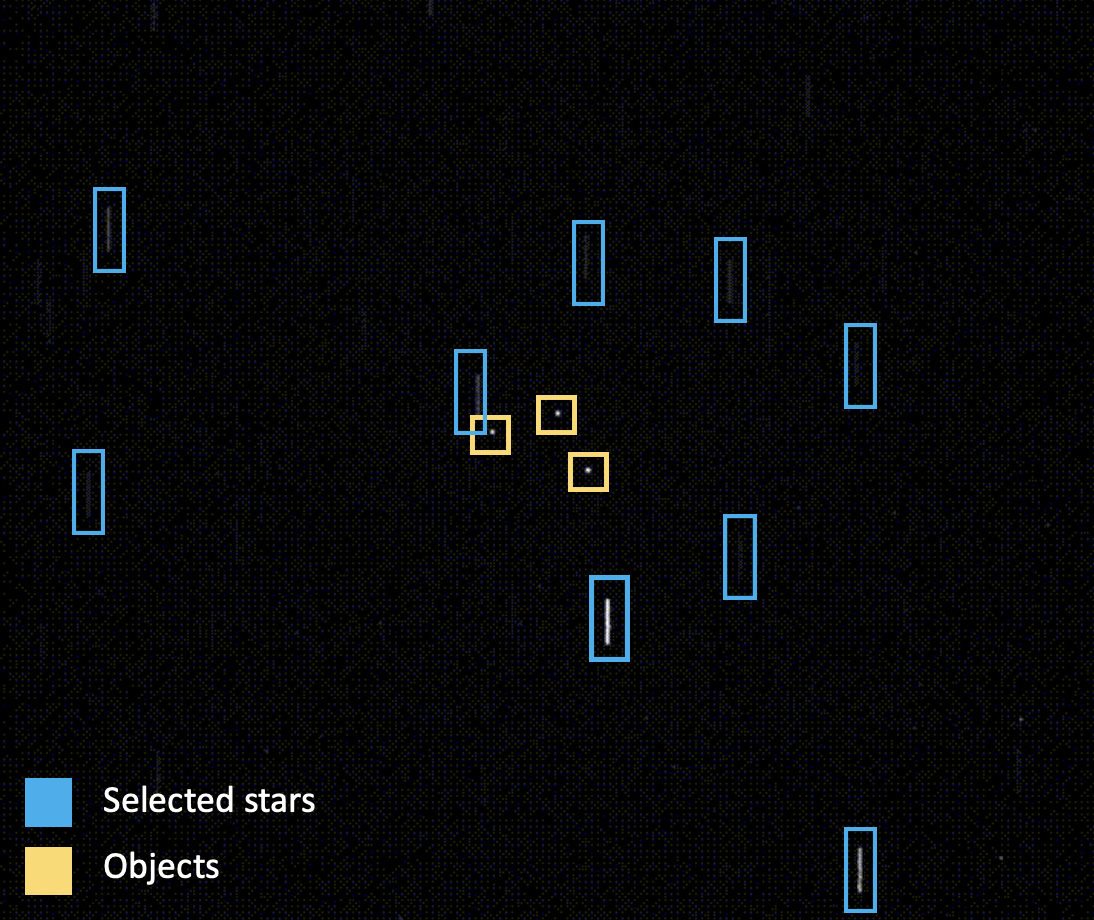
\includegraphics[width=\figmed]{static_images/static_pogs_annotated.png}
  \caption{Raw image of three GEO objects with stars streaking through the background. As expected, the star signals have a variety of signal-to-noise ratios. Taken by the Purdue Optical Ground station at \pogslla by Nathan Houtz.}
  \label{fig:pogs_observation_example}
\end{figure}

Krag \cite{krag2003} modeled this signal by building a $1^\circ \times 1^\circ$ grid of surface
brightness values for the full inertial sphere, parameterized by RA/Dec. Krag used the
Guide Star catalog, which contains 15 million stars down to apparent magnitude 16. Exponential extrapolation
was used to predict star counts in each bin for higher magnitudes \cite{krag2003}. Twenty years later, larger star catalogs exist that are nearly complete to much higher apparent magnitudes. The integrated
starlight catalog used in this work was built from the GAIA catalog with approximately 1.5 billion
stars down to magnitude 21-22 \cite{gaia_dr3}. The same $1^\circ \times 1^\circ$ grid was computed
using GAIA \cite{astroquery_gaia}, resulting in Figure
\ref{fig:gaiapatched} which shows the computed brightness map in units of $S_{10}$. 

\begin{figure}[ht]
  \centering
  \includegraphics[width=\figbig]{sphx_glr_gaia_patched_catalog_001_2_00x.png}
  \caption{Integrated starlight brightness map, produced from Gaia DR3 data \cite{gaia_dr3} using \cite{astroquery_gaia}}
  \label{fig:gaiapatched}
\end{figure}

With this map of exoatmospheric mean brightness of the night sky due to integrated
starlight, the corresponding signal mean in the telescope CCD is computed, adopting Krag's formulation \cite{krag2003}.

\begin{equation} \label{eq:bint}
 \mathcal{Z} = A_\mathrm{aperture}
  \int_{10^{-8}}^{10^{-6}}{ \mathcal{ZM}(\lambda) \cdot \textrm{QE}(\lambda) \cdot \textrm{ATM}(\lambda)
  \cdot \left( \frac{\lambda}{h c} \right) \: d\lambda}  
\end{equation}

In Eq \ref{eq:bint}, $D$ is the telescope aperture diameter in meters, $h$ is Plank's constant in
$\left[ \frac{m^2 kg}{s} \right]$, and $c$
is the speed of light in vacuum in $\left[ \frac{m}{s} \right]$. The resulting quantity
$\mathcal{Z}$ has units of $\left[ \frac{1}{s} \right]$, representing the mean total photons passing
through the telescope aperture due to integrated starlight. 

\begin{equation} \label{eq:starlight_adu}
  \bar{S}_{star} = 10^{-4} \cdot \mathcal{Z} \cdot \left( \frac{s_\mathrm{pix}}{3600} \right)^2 \cdot \Delta t \cdot
  b_{is}
\end{equation}

In Eq \ref{eq:starlight_adu}, $b_{is}$ is the integrated starlight brightness in $\left[ S_{10}
\right]$ computed by linearly interpolating the dataset in Figure \ref{fig:gaiapatched}, $s_\mathrm{pix}$ is the telescope pixel scale in $\left[ \frac{arcsecond}{pix} \right]$ and $\Delta t$ is the integration time in seconds. Note the addition of the $10^{-4}$ factor to reconcile catalog surface brightness in terms of 10th magnitude stars, and the 0th magnitude source in $\mathcal{Z}$. This yields $\bar{S}_{star}$ with units $\left[ \frac{e^-}{pix^2} \right]$; photoelectron counts (ADU) per pixel. Figure \ref{fig:starlight_hemi} shows the background signal mean due to integrated starlight.

\begin{figure}[ht]
  \centering
  \includegraphics[width=\figmed]{sphx_glr_background_signals_002.png}
  \caption{Integrated starlight signal on the local observer hemisphere. The observer is in New Mexico, USA at
  \pogslla}
  \label{fig:starlight_hemi}
\end{figure}

\subsubsection{Scattered Moonlight}

Moonlight scattering through the atmosphere significantly increases background brightness \cite{krag2003}. This scattering effect can be decomposed into Rayleigh (isotropically distributed) and Mie (exponentially distributed) scattering modes. The Rayleigh scattered component is computed with Table 4 published by Daniels parameterized by the angle from the observation to zenith $z_\mathrm{obs}$, the angle from the Moon to zenith $z_\mathrm{Moon}$, and the angle between the observation and the Moon on the horizon $\Delta Az$ \cite{daniels1977}. Interpolating this table yields the intensity of the Rayleigh scattering $F_{rs}$ in $10^{-10}$ $W/(cm^2 \cdot \mu m \cdot sr)$ \cite{krag2003}. The Mie scattered component is formulated \cite{krag2003}:

\begin{equation} \label{eq:mie_scattering_moon}
  F_{ms}(\lambda) = a_1 \left[ e^{-\left(\frac{\Psi}{\Psi_1}\right)} + a_2 e^{-\left(\frac{\pi - \Psi}{\Psi_2}\right)} \right] F_{rs}(\lambda).
\end{equation}

Daniels recommends $a_1 \in [50, 100]$, $a_2 \in [0.01, 0.02]$, $\Psi_1 \in [10^\circ, 20^\circ]$, and $\Psi_2 \approx 50$ \cite{daniels1977}. Prior to any station-specific fitting, the center of each interval is chosen, yielding $a_1 = 75$, $a_2 = 0.015$, $\Psi_1 = 15^\circ$, and $\Psi_2 = 50^\circ$. $a_1$ and $a_2$ are dimensionless, such that $F_{ms}$ also has units of $10^{-10}$ $W/(cm^2 \cdot \mu m \cdot sr)$. The total intensity of the scattered moonlight $F_{mt}$ following Krag's formulation \cite{krag2003}:

\begin{equation} \label{eq:total_scattered_moonlight}
  F_{mt} = f(\theta) \left[ F_{rs}(\lambda) + F_{ms}(\lambda) \right].
\end{equation}

in Eq \ref{eq:total_scattered_moonlight}, $f(\theta)$ is the lunar phase function which describes the fraction of the full Moon brightness reflected at an observer when the Sun-Moon-observer angle is $\theta$. This function is linearly interpolated within Table 3 in \cite{daniels1977}. Finally, Krag introduces a correction factor $f_{corr}$ to account for the difference between the Sun's irradiance spectrum and the spectrum of scattered moonlight, defined to be \cite{krag2003}:

\begin{equation} \label{eq:krag_f_corr}
  f_{corr} = \frac{I_s}{\textrm{SUN}(550 \: \left[\textrm{nm}\right])}.
\end{equation}

With all these pieces, the mean scattered moonlight signal in ADU per pixel is \cite{krag2003}:

\begin{equation} \label{eq:moonlight_adu}
  \bar{S}_\mathrm{Moon} = F_{mt}(550 \: \left[\textrm{nm}\right]) \cdot \mathcal{S}_\mathrm{int} \cdot \left( \frac{s_\mathrm{pix}}{3600} \right)^2 \cdot \Delta t \cdot f_{corr}.
\end{equation}

\begin{figure}[ht]
  \centering
  \includegraphics[width=\figmed]{sphx_glr_background_signals_001.png}
  \caption{Mean scattered moonlight signal on the local observer hemisphere. The observer is in New Mexico, USA at
  \pogslla}
  \label{fig:moonlight_hemi}
\end{figure}

\subsubsection{Zodiacal Light}

Zodiacal light is an effect created by sunlight reflecting off of dust in the ecliptic plane \cite{krag2003}. Zodiacal light is strongest around the Sun --- an exclusion zone for most optical telescopes --- but also reaches a peak directly away from the Sun due to the opposition effect. This peak is known as the Gegenschein, meaning "opposing light". The zodiacal light brightness is linearly interpolated within Table 1 of \cite{roach1972} which is listed for convenience in Appendix \ref{data:roach_zod}. This reports the surface brightness of the zodiacal light $B_\mathrm{zod}(\alpha, \delta)$ in $S_{10}$, which is used without conversion to find the mean CCD signal in ADU per pixel via:

\begin{equation} \label{eq:zodiacal_adu}
  \bar{S}_{zod} = \mathcal{Z} \cdot \left( \frac{s_\mathrm{pix}}{3600} \right)^2 \cdot \Delta t \cdot B_\mathrm{zod}(\alpha, \delta) \cdot 10^{-4}.
\end{equation}

As in the integrated starlight signal, the $10^{-4}$ factor reconciles the $S_{10}$ surface brightness with the 0th magnitude source in $\mathcal{Z}$. 

\begin{figure}[ht]
  \centering
  \includegraphics[width=\figmed]{sphx_glr_background_signals_004.png}
  \caption{Mean zodiacal light signal on the local observer hemisphere. The observer is in New Mexico, USA at
  \pogslla}
  \label{fig:zod_hemi}
\end{figure}

\subsubsection{Background Sampling}

The background signals are only defined in terms of their means, as each signal models the expected amount of radiation without accounting for the quantized nature of light \cite{krag2003}. Since light is transmitted in individual photons, their incidence on a given pixel will follow a statistical distribution. Assuming that each photon does not interact with others, the incidence of a photon on a pixel is well modeled as a Poisson process for each background term \cite{frueh2019notes}. This distribution models the number of independent and identically distributed events that occur during a time period. For CCD astronomy, this translates to the event of a photon hitting the sensor. A Poisson distribution is defined on the positive integers by a single parameter $\lambda$ which is both the mean and variance of the distribution. The probability density function (PDF) for the Poisson distribution takes the form \cite{frueh2019notes}:

\begin{equation} \label{eq:poisson_pdf}
  P_\lambda(x=k) = \frac{\lambda^k e^{-\lambda}}{k!}.
\end{equation}

This distribution has a useful property that $P_{\lambda_1 + \lambda_2}(x=k) = P_{\lambda_1}(x=k) + P_{\lambda_2}(x=k)$ so long as the distributions described by $\lambda_1$ and $\lambda_2$ are independent. The background sources modeled in this work are reasonably assumed to be independent as they each originate from distinct physical processes.

\begin{equation} \label{eq:background_poisson}
  \lambda_\mathrm{background} = \bar{S}_{airglow} + \bar{S}_{pollution} + \bar{S}_{twilight} + \bar{S}_{star} + \bar{S}_\mathrm{Moon} + \bar{S}_{zod}
\end{equation}

Drawing samples from the Poisson distribution defined by $\lambda_\mathrm{background}$ computes the background of the CCD image. 

\subsection{Sensor Effects}

CCD sensors accumulate noise during both the integration time and readout phases. Characterizing these noise sources is necessary to sample realistic light curves and compute the signal-to-noise ratio of the measurements.

\subsubsection{Dark Noise}

The dark noise, also called the dark current or dark count, captures the temperature-dependent accumulation of electrons in the CCD pixel wells \cite{krag2003}. This noise source is modeled as a Poisson process with parameter $\lambda_{dark}$ \cite{frueh2019notes} and is assumed to be independent from the other sensor effects. This source accumulates with the integration time, giving it units of counts per second \cite{krag2003}.

\subsubsection{Readout Noise}

When the CCD is read out, the charge contained in each pixel well must be digitized. This process introduces noise in the final signal due to electronic effects within the CCD circuitry and its surrounding environment \cite{krag2003}. The readout noise is modeled as a zero-mean Gaussian distribution with variance $\sigma_\mathrm{read}^2$ and is also assumed to be independent from other sensor effects \cite{frueh2019notes}.

\subsubsection{Truncation Noise}

Truncation noise in a CCD stems from the fact that the charge in each pixel is digitized into an integer factor of the gain \cite{frueh2019notes}. This is modeled using a uniform distribution on $\left[ -g/2, g/2 \right]$, yielding a variance $N^2_\mathrm{trunc} = \frac{g^2}{24}$ \cite{frueh2019notes}.

The particular noise variances for the Purdue Optical Ground Station are listed in \ref{tb:pogs_parameters}.

\subsection{Observer Constraints}

Accurately simulating light curves requires realistic constraints on the observing station. For an optical ground station, basic operational constraints include local eclipse, target SNR, Moon exclusion angle, and minimum elevation constraints. This section develops these constraints.

\subsubsection{Earth Penumbra}

The Earth casts a conical shadow into space. Outside this shadow, the fraction of received solar irradiance $f_{Sun}$ is assumed to be $1$. Inside the shadow, the central region of zero received solar irradiance $f_{Sun}=0$ is known as umbra, while the boundary between umbra and full Sun is known as the penumbra where $f_{Sun} \in (0,1)$. The precise gradient of the penumbra is defined by the geometry of the overlapping Earth and Sun disks from the perspective of the object. Given the position of the Sun $\vctr{r}_{Sun}$ computed following Section \ref{sec:planet_ephem} and object in J2000, the local irradiance fraction is expressed \cite{krag2003}:

\begin{align*} \numberthis \label{eq:irradiance_fraction_angles}
  \vctr{r}_{obj \rightarrow Sun} &= \vctr{r}_{Sun} - \vctr{r}_\mathrm{obj} \\
  \epsilon_s &= \sin^{-1}\left( \frac{R_{Sun}}{\| \vctr{r}_{obj \rightarrow Sun} \|} \right) \\
  \epsilon_e &= \sin^{-1}\left( \frac{R_\mathrm{Earth}(\phi_\mathrm{obj})}{\| \vctr{r}_\mathrm{obj} \|} \right) \\
  \epsilon &= \cos^{-1} \left( -\hat{r}_{obj \rightarrow Sun} \cdot \hat{r}_\mathrm{obj} \right) \\
  \epsilon_1 &= \frac{\epsilon^2 - \epsilon_e^2 + \epsilon_s^2}{2 \epsilon} \\
  \epsilon_2 &= \frac{\epsilon^2 + \epsilon_e^2 - \epsilon_s^2}{2 \epsilon}. \\
\end{align*}

\graphicspath{{/Users/liamrobinson/Documents/msthesis/static_images}}
\begin{figure}[!htb]
  \centering
  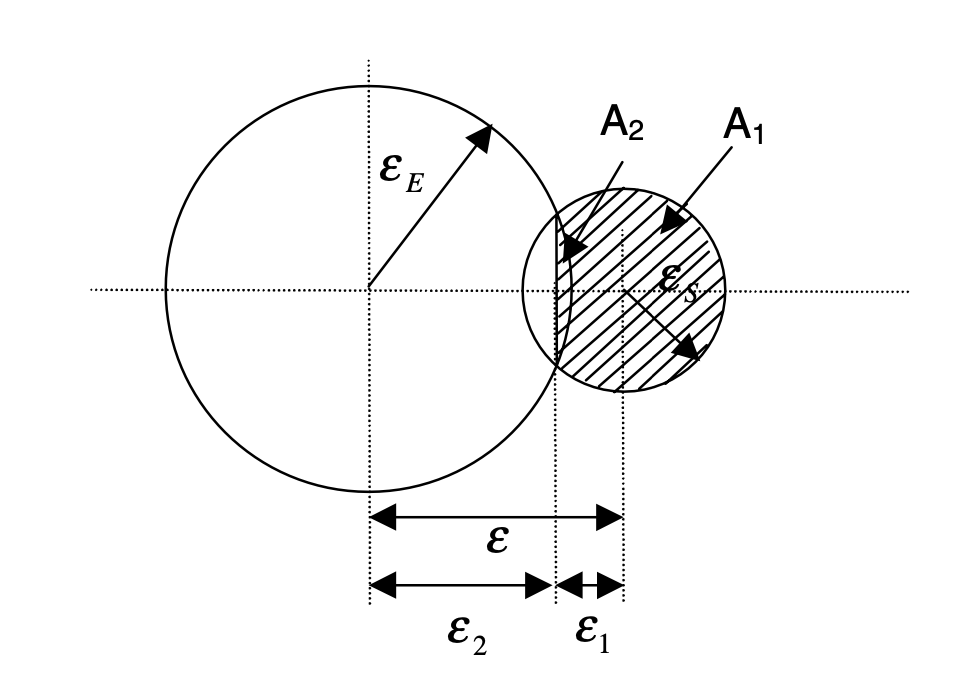
\includegraphics[width=\figmed]{angle_defs_krag_520.png}
  \caption{Angle and area definitions for penumbra shadowing, Figure 5.20 in \cite{krag2003}}
  \label{fig:penumbra_angles}
\end{figure}
\graphicspath{{/Users/liamrobinson/Documents/msthesis/static_images/aas_2022_figs}}

In Eq \ref{eq:irradiance_fraction_angles}, $\vctr{r}_{obj \rightarrow Sun}$ is the vector from the object to the Sun in J2000, $\epsilon_s$ is the half-angle of the Sun disk at the object, $\epsilon_e$ is the half-angle of the Earth disk from the object as a function of the geodetic latitude of the object $\phi_\mathrm{obj}$. Additionally, $\epsilon$ is the angle between the center of the Earth and Sun from the perspective of the object, with $\epsilon_1$ and $\epsilon_2$ being the angles from the center of the Sun and Earth disks to the center of their overlap, if it exists \cite{krag2003}. These angles are defined in Figure \ref{fig:penumbra_angles}. Given these angles, the illumination fraction $f_{Sun}$ is computed:

\begin{equation} \label{eq:irradiance_fraction}
  f_{Sun} = \begin{cases}
    1 & \epsilon \geq (\epsilon_s + \epsilon_e) \\ 
    0 & \epsilon \leq (\epsilon_e - \epsilon_s) \\ 
    \frac{a_1 - a_2}{\pi \epsilon_s^2} & \mathrm{else}
  \end{cases}.
\end{equation}

In Eq \ref{eq:irradiance_fraction}, the solid angles $a_1$ and $a_2$ are defined in Figure \ref{fig:penumbra_angles} and are computed via:

\begin{align*} \numberthis \label{eq:penumbra_areas}
  a_1 &= \pi \epsilon_s^2 - \epsilon_s^2 \cos^{-1} \left(\frac{\epsilon_1}{\epsilon_s}\right)
    + \epsilon_1 \sqrt{\epsilon_s^2 - \epsilon_1^2} \\
  a_2 &= \epsilon_e^2 \cos^{-1}\left(\frac{\epsilon_2}{\epsilon_e} \right) - \epsilon_2 \sqrt{\epsilon_e^2 - \epsilon_2^2} \\
\end{align*}

Computing Eq \ref{eq:irradiance_fraction} for a dense grid of points in the J2000 reference frame reveals the geometry of the penumbra and umbra in Figure \ref{fig:penumbra}, illustrating that the penumbra expands into the umbra as the observer recedes from the Earth. 

\graphicspath{{/Users/liamrobinson/Documents/PyLightCurves/docs/build/html/_images}}
\begin{figure}[!htb]
  \centering
  \includegraphics[width=\figbig]{sphx_glr_penumbra_plane_001.png}
  \caption{Shadow fraction in J2000, effect exaggerated by scaling the Sun radius by a factor $10$}
  \label{fig:penumbra}
\end{figure}
\graphicspath{{/Users/liamrobinson/Documents/msthesis/static_images/aas_2022_figs}}

\subsubsection{SNR}

As the signal-to-noise ratio of an object signal on the CCD pixel grid degrades, it becomes more difficult to determine whether an object is present at all. Given a minimum limiting SNR $\mathrm{SNR}_{min}$ this constraint takes the form:

\begin{equation} \label{eq:snr_exclusion}
  \nu_{\mathrm{SNR}} = \begin{cases}
    1 & \mathrm{SNR} > \mathrm{SNR}_{min}\\
    0 & \mathrm{else}
  \end{cases}.
\end{equation}

In Eq \ref{eq:snr_exclusion}, $\nu_{\mathrm{SNR}} = 1$ implies that the observation is valid, with $\nu_{\mathrm{SNR}} = 0$ implying that the object signal cannot be discerned from the image background.

\subsubsection{Moon Exclusion Angle}

Focusing the irradiance of the Moon onto the sensor grid will seriously damage the CCD. For the Purdue Optical Ground Station, stray light from the Moon begins leaking into the optics around $30^\circ$ from the center of the Moon disk. This observation constraint is imposed for an arbitrary exclusion angle $\theta_{Moon,ex}$ via:

\begin{equation} \label{eq:moon_exclusion}
  \nu_\mathrm{Moon} = \begin{cases}
    1 & \cos^{-1}\left( \frac{\left( \vctr{r}_\mathrm{Moon} - \vctr{r}_\mathrm{obs} \right) \cdot \left( \vctr{r}_\mathrm{obj} - \vctr{r}_\mathrm{obs} \right)}{\| \vctr{r}_\mathrm{Moon} - \vctr{r}_\mathrm{obs} \| \| \vctr{r}_\mathrm{obj} - \vctr{r}_\mathrm{obs} \|} \right) > \theta_{Moon,ex}\\
    0 & \mathrm{else}
  \end{cases}.
\end{equation}

In Eq \ref{eq:moon_exclusion}, $\nu_\mathrm{Moon} = 1$ implies that the observation is valid, with $\nu_\mathrm{Moon} = 0$ implying that the observation is too close to the Moon. $\vctr{r}_\mathrm{Moon}$ should be computed with SPICE following Section \ref{sec:planet_ephem}.

\subsubsection{Minimum Elevation}

Due to the local topology at the observer location, an operator may assign a minimum angle from the horizon $\theta_{elev,min}$ for observations. Approximating the station inertial position $\vctr{r}_\mathrm{obs}$ as being aligned with zenith, this yields the condition:


\begin{equation} \label{eq:elevation_exclusion}
  \nu_{elevation} = \begin{cases}
    1 & 90^\circ - \cos^{-1}\left( \frac{\left( \vctr{r}_\mathrm{obj} - \vctr{r}_\mathrm{obs} \right) \cdot \left( \vctr{r}_\mathrm{obs} \right)}{\| \vctr{r}_\mathrm{Moon} - \vctr{r}_\mathrm{obs} \| \| \vctr{r}_\mathrm{obs} \|} \right) > \theta_{elev,min}\\
    0 & \mathrm{else}
  \end{cases}.
\end{equation}

In Eq \ref{eq:elevation_exclusion}, $\nu_{elevation} = 1$ implies that the observation is valid, with $\nu_{elevation} = 0$ implying that the observation is too close to the horizon.

\subsection{Mean Irradiance at The Observer}

Given the normalized irradiance computed via Eq \ref{eq:lc_func_normalized} for convex objects or Eq \ref{eq:lc_normalized_engine} for any object shaded using Algorithm \ref{alg:pix_shading}, the received mean irradiance at the telescope aperture is given by:

\begin{equation} \label{eq:mean_irrad_at_aperture}
  \bar{I} = \nu_{Moon,ex} \cdot \nu_{elevation} \cdot \nu_{\mathrm{SNR}} \frac{I_s f_{Sun} \check{I}}{\left( \vctr{r}_\mathrm{obj} - \vctr{r}_\mathrm{obs} \right)^2}.
\end{equation}

In Eq \ref{eq:mean_irrad_at_aperture}, the conditions $\nu_{Moon,ex},\: \nu_{elevation},\: \nu_{\mathrm{SNR}}$ determine whether the telescope can take the observation and identify the object in the image, $I_s f_{Sun}$ determines the solar irradiance incident on the object, and the remaining terms $\check{I} / \left( \vctr{r}_\mathrm{obj} - \vctr{r}_\mathrm{obs} \right)^2$ dimensionalize the normalized irradiance. In order to sample a noisy light curve, this mean irradiance must be converted into a mean photoelectron count via Eq \ref{eq:irrad_to_count}, yielding $\bar{C}_\mathrm{all}$:

\begin{equation}
  \bar{C}_\mathrm{all} = \mathcal{S}_\mathrm{int} \cdot \bar{I} \cdot \Delta t.
\end{equation}

\subsection{Sampling Noisy Light Curves} \label{sec:sampling_lcs}

Given the irradiance of the object observed by the telescope, the noisy light curve is computed by building a grid containing the object signal, background noise, and sensor noise. On a pixel-by-pixel basis, the mean object signal is given by an alteration of Eq \ref{eq:airy_gaussian} where the angle $\theta$ from the center of the frame is converted into pixels via $\theta^2 = \left((x - x_0)^2 + (y - y_0)^2 \right) / s_\mathrm{pix}^2$:

\begin{equation} \label{eq:obj_signal_grid}
  \bar{C}_\mathrm{obj}(x, y) = \frac{0.838 \bar{C}_\mathrm{all}}{2 \pi \sigma^2} \exp\left( - \frac{(x - x_0)^2 + (y - y_0)^2}{2 \sigma^2  s_\mathrm{pix}^2} \right).
\end{equation}

In Eq \ref{eq:obj_signal_grid}, $\left(x_0, y_0\right)$ are the exact pixel coordinates of the object centroid, $\sigma$ is the Gaussian standard deviation from Eq \ref{eq:airy_variance} in arcseconds, and $s_\mathrm{pix}$ is the pixel scale in arcseconds per pixel. Likewise, the total noise sampled in each pixel is given by samples from all the relevant source distributions:

\begin{equation} \label{eq:noise_signal_grid}
  C_{noise} = N_\mathrm{background} + N_{dark} + N_\mathrm{trunc} + N_\mathrm{read}.
\end{equation}

In Eq \ref{eq:noise_signal_grid}, $N_\mathrm{background}$ is a sample drawn from $\mathrm{Pois}(\lambda_\mathrm{background})$, $N_{dark}$ is drawn from $\mathrm{Pois}(\Delta t \cdot \lambda_{dark})$, $N_\mathrm{trunc}$ is drawn from $\mathrm{Uniform}(-g/2, g/2)$, and $N_\mathrm{read}$ is drawn from $\mathrm{N}(0, \sigma_\mathrm{read}^2)$. 

Assuming perfect knowledge of the image background mean in the region around the object signal --- a reasonable assumption given that there are generally millions of background pixels in the image --- the counts $C_{obj,meas}$ attributed to the object pixels $\{x_\mathrm{obj}, y_\mathrm{obj}\}$ is given by:

\begin{align*} \numberthis \label{eq:noisy_counts}
  C_{noise,all} &= \sum_{i=1}^{A_\mathrm{Airy}}{C_{noise,i}} \\
  C_{obj,all} &= \sum_{x \in x_\mathrm{obj}, \: y \in x_\mathrm{obj}}{\bar{C}_\mathrm{obj}(x, y)} \\
  C_{obj,meas} &= C_{noise,all} - A_\mathrm{Airy} \left( \Delta t \cdot \lambda_{dark} + \lambda_\mathrm{background} \right) 
\end{align*}

In Eq \ref{eq:noisy_counts}, $A_\mathrm{Airy}$ is the area of the central maximum of the Airy disk in square pixels presented in Eq \ref{eq:airy_area}. The measured object signal $C_{obj,meas}$ can then be transformed into irradiance via Eq \ref{eq:count_to_irrad}:

\begin{equation} \label{eq:noisy_counts_to_irrad}
  I_{obj,meas} = \frac{C_{obj,meas}}{\mathrm{\mathcal{S}_\mathrm{int}} \cdot \Delta t}
\end{equation}

or to apparent magnitude by applying Eq \ref{eq:mag_to_irradiance}:

\begin{equation}
  m_{obj,meas} = -2.5 \log_{10}\left( \frac{I_{obj,meas}}{I_0} \right)
\end{equation}

or normalized irradiance by applying Eq \ref{eq:irradiance_to_norm_irradiance}:

\begin{equation} \label{eq:ihat_meas}
  \check{I}_{obj,meas} = \frac{\| \vctr{r}_\mathrm{obj} - \vctr{r}_\mathrm{obs} \|^2}{I_s} I_{obj,meas}.
\end{equation}

\section{Light Curve Simulation Results}

\subsection{Case 1: Normalized Light Curve of a Simple Object}

This section presents the entire process for simulating the normalized light curve of a simple object. To begin, the properties of the object and the observing station are defined in Table \ref{tb:case1_obj_props}. The cube model used for this case is displayed in Figure \ref{fig:case1_obj}.

\begin{table}[]
  \centering
  \begin{tabular}{|l|l|}
  \hline
  \textbf{Parameter} & \textbf{Value} \\ \hline
  Object & \texttt{cube.obj} \ref{sec:obj_listing} \\ \hline
  SATNUM & $36411$ \\ \hline
  $\vctr{q}_0$ & $\left[ 0, 0, 0, 1 \right]^T$ \\ \hline
  $w_0$ & $\left[ 0.04082483, 0.08164966, 0.04082483 \right]^T$ $[rad/s]$ \\ \hline
  $J$ & $\mathrm{diag}\left( 1.0, 2.0, 3.0 \right)$ $\left[ kg \cdot m^2 \right]$ \\ \hline
  BRDF & Phong \\ \hline
  $C_s$ & $0.3$ \\ \hline
  $C_d$ & $0.7$ \\ \hline
  $n$ & $5$ \\ \hline
  Initial date & 2023-03-26 05:00:00 UTC \\ \hline
  $\Delta t$ & $0.1$ $[s]$ \\ \hline
  $n_\mathrm{obs}$ & $360$ $[s]$ \\ \hline
  $\phi_{geod}$ & $32.900^\circ$ \\ \hline
  $\lambda$ & $-105.533^\circ$ \\ \hline
  \end{tabular}
  \caption{Object and station simulation parameters for case 1}
  \label{tb:case1_obj_props}
\end{table}

\graphicspath{{/Users/liamrobinson/Documents/PyLightCurves/docs/build/html/_images}}
\begin{figure}[!htb]
  \centering
  \includegraphics[width=\figmed]{sphx_glr_light_curves_types_001.png}
  \caption{Cube model for case 1}
  \label{fig:case1_obj}
\end{figure}

To begin, the position of the object in TEME is computed using SGP4. That position is converted to ICRF using Eqs \ref{eq:teme_to_tod}, \ref{eq:tod_to_mod}, and \ref{eq:mod_to_icrf}. The position of the station in ITRF is computed using Eq \ref{eq:lla_to_itrf} and converted to ICRF using Eqs \ref{eq:itrf_to_gtod}, \ref{eq:gtod_to_teme}, \ref{eq:teme_to_tod}, \ref{eq:tod_to_mod}, and \ref{eq:mod_to_icrf}. The position of the Sun is determined with SPICE following Section \ref{sec:planet_ephem}. 

The attitude profile of the object is propagated with Eqs \ref{eq:rbtf_dynamics} and \ref{eq:quat_kde} using $\vctr{M}=\mathbf{0}$ for torque free rigid body motion. The resulting attitude time history produces $\vctr{\vctr{q}(t)}$, $\vctr{\vctr{\omega}(t)}$, as well as the body frame vectors from the object to the Sun and observer depicted in Figure \ref{fig:case1_attitude}.

\begin{figure}[!htb]
  \centering
  \includegraphics[width=\textwidth]{sphx_glr_light_curves_types_002_2_00x.png}
  \caption{Attitude time history for case 1}
  \label{fig:case1_attitude}
\end{figure}

Next, the BRDF is used to compute the reflection matrix for the cube with Eq \ref{eq:reflection_matrix}. The normalized light curve is simply computed with Eq \ref{eq:lc_func_normalized}, using Eq \ref{eq:brdf_phong} and noting that $\mu_{ij} = 0$ as the object is convex. This yields the normalized light curve depicted in Figure \ref{fig:case1_lc}.

\begin{figure}[!htb]
  \centering
  \includegraphics[width=\figmed]{sphx_glr_light_curves_types_004_2_00x.png}
  \caption{Normalized light curve for case 1}
  \label{fig:case1_lc}
\end{figure}

Figure \ref{fig:case1_lc} has a few important features to recognize. Some sections of the light curve are flat, indicating that all illuminated faces are orthogonal to each other and reflecting diffusely. When one of the face normal vectors approaches the halfway vector $H$, a specular glint occurs, leading to a temporary sharp increase in the light curve value. Overall, this is exactly the behavior expected given the observation conditions.

\subsection{Accurate Satellite Models}

To produce accurate light curves for real space objects, 3D model files were collected and tuned for use with the light curve simulator. These models are shown in Figure \ref{fig:satellite_lineup}. Each model is correctly scaled, with accurate material properties applied to their faces. Figure \ref{fig:satellite_lineup} highlights the size of the GEO communications satellites (TELSTAR, HYLAS, Hispasat, and ASTRA). In contrast, the LEO satellites (Starlink and Landsat) are dwarfed at the left end of the lineup.

\begin{figure}[ht]
    \centering
    \includegraphics[width=\figbig]{sphx_glr_satellite_lineup_001.png}
    \caption{Selected space objects with soccer field for size reference. In order, the objects are TESS, Starlink V1, TDRS, Landsat 8, Hispasat 30W-6, Saturn V SII, TELSTAR 19V, HYLAS 4, and simplified ASTRA.
    }
    \label{fig:satellite_lineup}
\end{figure}

\subsection{Case 2: Realistic Light Curve for a Box-Wing Satellite} \label{sec:case2}

The second case deals with simulating a realistic noisy light curve for a complex, nonconvex satellite model with observer constraints. Table \ref{tb:case2_obj_props} summarizes the simulation parameters for the object and station. The object geometry is displayed in Figure \ref{fig:case2_obj}.

\begin{table}[]
  \centering
  \begin{tabular}{|l|l|}
  \hline
  \textbf{Parameter} & \textbf{Value} \\ \hline
  Object & \href{https://raw.githubusercontent.com/liamrobinson1/Light-Curve-Models/main/accurate_sats/matlib_goes17.obj}{goes17.obj} \\ \hline
  SATNUM & $32711$ \\ \hline
  $\vctr{q}_0$ & $\left[ 0, 0, 0, 1 \right]^T$ \\ \hline
  $w_0$ & $\left[ 0.00707107, 0.,         0.00707107 \right]^T$ $[rad/s]$ \\ \hline
  $J$ & $\mathrm{diag}\left( 1.0, 2.0, 2.0 \right)$ $\left[ kg \cdot m^2 \right]$ \\ \hline
  BRDF & Phong \\ \hline
  Initial date & 2022-12-09 08:00:00 UTC \\ \hline
  $\Delta t$ & $10$ $[s]$ \\ \hline
  $n_\mathrm{obs}$ & $180$ $[s]$ \\ \hline
  Telescope & Table \ref{tb:pogs_parameters} \\ \hline
  $\phi_{geod}$ & $32.900^\circ$ \\ \hline
  $\lambda$ & $-105.533^\circ$ \\ \hline
  $SNR_{min}$ & $3$ \\ \hline
  $\theta_{Moon,ex}$ & $30^\circ$ \\ \hline
  $\theta_{elev,min}$ & $15^\circ$ \\ \hline
  \end{tabular}
  \caption{Object and station simulation parameters for case 2}
  \label{tb:case2_obj_props}
\end{table}

\begin{figure}[!htb]
  \centering
  \includegraphics[width=\figmed]{sphx_glr_light_curves_types_005.png}
  \caption{GOES 17 model for case 2}
  \label{fig:case2_obj}
\end{figure}

To begin, the position of the object in TEME is computed using SGP4. That position is converted to ICRF using Eqs \ref{eq:teme_to_tod}, \ref{eq:tod_to_mod}, and \ref{eq:mod_to_icrf}. The position of the station in ITRF is computed using Eq \ref{eq:lla_to_itrf} and converted to ICRF using Eqs \ref{eq:itrf_to_gtod}, \ref{eq:gtod_to_teme}, \ref{eq:teme_to_tod}, \ref{eq:tod_to_mod}, and \ref{eq:mod_to_icrf}. The position of the Sun is determined with SPICE following Section \ref{sec:planet_ephem}. 

The attitude profile of the object is propagated with Eqs \ref{eq:rbtf_dynamics} and \ref{eq:quat_kde} using $\vctr{M}=\mathbf{0}$ for torque free rigid body motion. The resulting attitude time history produces $\vctr{\vctr{q}(t)}$, $\vctr{\vctr{\omega}(t)}$, as well as the body frame vectors from the object to the Sun and observer depicted in Figure \ref{fig:case2_attitude}.

\begin{figure}[!htb]
  \centering
  \includegraphics[width=\textwidth]{sphx_glr_light_curves_types_006_2_00x.png}
  \caption{Attitude time history for case 2}
  \label{fig:case2_attitude}
\end{figure}

The BRDF --- which varies across the surface of the object --- is encoded in the \texttt{.obj} file in the red channel of the diffuse material color $R$ such that $C_d = R$ and $C_s = 1 - R$. Given the unit vectors in the object body frame pointing towards the observer and the Sun, Algorithms \ref{alg:depth_map} and \ref{alg:pix_shading} are used to render images of the object which are integrated to yield a mean normalized irradiance value $\check{I}$ with Eqs \ref{eq:ortho_area} and \ref{eq:lc_normalized_engine}. 

This normalized irradiance is dimensionalized with Eq \ref{eq:irradiance_to_norm_irradiance} to yield a mean irradiance $I$. Next, the background signal variances are computed for the Moonlight in Eq \ref{eq:moonlight_adu}, zodiacal light in Eq \ref{eq:zodiacal_adu}, integrated starlight in Eq \ref{eq:starlight_adu}, twilight in eq \ref{eq:twilight_adu}, light pollution in Eq \ref{eq:pollution_adu}, and airglow in Eq \ref{eq:airglow_adu}. These background signal variances are used to compute the overall background variance $\lambda_\mathrm{background}$. The signal variance due to read noise, dark noise, and truncation noise are found in Table \ref{tb:pogs_parameters}, yielding the overall mean and variance of the background pixels. 

These means and variances are used to compute the SNR of each attempted observation using Eq \ref{eq:ccd_snr}. This SNR is used compute the minimum SNR constraint in Eq \ref{eq:snr_exclusion}. The Moon exclusion angle constraint is also evaluated with Eq \ref{eq:moon_exclusion} and the minimum elevation constraint is evaluated with Eq \ref{eq:elevation_exclusion}. If all constraints are satisfied, the object is observable and the light curve measurement process can continue. Otherwise, the measurement is impossible and no value is saved for this timestep.

The mean value of the total photoelectron counts due to the object signal is computed from the mean irradiance $I$ using Eq \ref{eq:irrad_to_count} using the telescope parameters in Table \ref{tb:pogs_parameters}. This total mean count is then distributed across the CCD pixel grid using Eq \ref{eq:obj_signal_grid}. Now that all mean values are known, samples from the Poisson, Gaussian, and uniform distributions are sampled pixel-by-pixel to yield a final background and object signal on the CCD grid. The noisy light curve in ADU is then computed with Eq \ref{eq:noisy_counts} and transformed back to irradiance with Eq \ref{eq:noisy_counts_to_irrad}, depicted in Figure \ref{fig:case2_lc}.

\begin{figure}[!htb]
  \centering
  \includegraphics[width=\figmed]{sphx_glr_light_curves_types_007_2_00x.png}
  \caption{Light curve for case 2, produced with an object scale factor of $1/10$ to exaggerate noise}
  \label{fig:case2_lc}
\end{figure}

Figure \ref{fig:case2_lc} possesses a few important characteristics to note when compared to the results from case 1 in Figure \ref{fig:case1_lc}. The light curve for case 2 is much more complex, with higher frequency variation in the mean due to the many small geometric features making up the satellite model. As in the cube light curve, specular peaks are still evident around $260$ and $1050$ seconds after the simulation epoch. The noise is clearly seen in the regions shaded by standard deviation. As a result of this noise, the lower magnitude signals regions --- where little specular reflection is occurring --- are much more corrupted by the noise as its standard deviation represents a larger fraction of the signal magnitude. Importantly, these regions possess high-frequency oscillations in the mean that are highly obscured in any one sampling due to the additive noise. This highlights the importance of specular reflection for extracting reliable accurate features by pinpointing the normal vectors of certain faces by reaching above the noise. It must be noted that Figure \ref{fig:case2_lc} was produced with a scale factor of $1/10$ applied to the vertices of the GOES 17 3D model to make the effect of the noise more clear. In reality, large GEO objects like GOES should produce light curves with much less noise on the signal, as predicted by the simulator developed in this work. 